%%%%%%%%%%%%%%%%%%%%%%%%%%%%%%%%%%%%%%%%%
% Arsclassica Article
% LaTeX Template
% Version 1.1 (1/8/17)
%
% This template has been downloaded from:
% http://www.LaTeXTemplates.com
%
% Original author:
% Lorenzo Pantieri (http://www.lorenzopantieri.net) with extensive modifications by:
% Vel (vel@latextemplates.com)
%
% License:
% CC BY-NC-SA 3.0 (http://creativecommons.org/licenses/by-nc-sa/3.0/)
%
%%%%%%%%%%%%%%%%%%%%%%%%%%%%%%%%%%%%%%%%%

%----------------------------------------------------------------------------------------
%	PACKAGES AND OTHER DOCUMENT CONFIGURATIONS
%----------------------------------------------------------------------------------------

\documentclass[
12pt, % Main document font size
a4paper, % Paper type, use 'letterpaper' for US Letter paper
oneside, % One page layout (no page indentation)
%twoside, % Two page layout (page indentation for binding and different headers)
headinclude,footinclude, % Extra spacing for the header and footer
BCOR5mm, % Binding correction
]{scrartcl}
\usepackage[english]{babel}
\usepackage{url}
\usepackage{graphicx}
\usepackage{subcaption}
\usepackage{float}
\usepackage{epigraph}
\usepackage{mathcomp}
\usepackage{textcomp}
%%%%%%%%%%%%%%%%%%%%%%%%%%%%%%%%%%%%%%%%%
% Arsclassica Article
% Structure Specification File
%
% This file has been downloaded from:
% http://www.LaTeXTemplates.com
%
% Original author:
% Lorenzo Pantieri (http://www.lorenzopantieri.net) with extensive modifications by:
% Vel (vel@latextemplates.com)
%
% License:
% CC BY-NC-SA 3.0 (http://creativecommons.org/licenses/by-nc-sa/3.0/)
%
%%%%%%%%%%%%%%%%%%%%%%%%%%%%%%%%%%%%%%%%%

%----------------------------------------------------------------------------------------
%	REQUIRED PACKAGES
%----------------------------------------------------------------------------------------

\usepackage[
nochapters, % Turn off chapters since this is an article        
beramono, % Use the Bera Mono font for monospaced text (\texttt)
eulermath,% Use the Euler font for mathematics
pdfspacing, % Makes use of pdftex’ letter spacing capabilities via the microtype package
dottedtoc % Dotted lines leading to the page numbers in the table of contents
]{classicthesis} % The layout is based on the Classic Thesis style

\usepackage{arsclassica} % Modifies the Classic Thesis package

\usepackage[T1]{fontenc} % Use 8-bit encoding that has 256 glyphs

\usepackage[utf8]{inputenc} % Required for including letters with accents

\usepackage{graphicx} % Required for including images
\graphicspath{{Figures/}} % Set the default folder for images

\usepackage{enumitem} % Required for manipulating the whitespace between and within lists

\usepackage{lipsum} % Used for inserting dummy 'Lorem ipsum' text into the template

%\usepackage{subfig} % Required for creating figures with multiple parts (subfigures)

\usepackage{amsmath,amssymb,amsthm} % For including math equations, theorems, symbols, etc

\usepackage{varioref} % More descriptive referencing

%----------------------------------------------------------------------------------------
%	THEOREM STYLES
%---------------------------------------------------------------------------------------

\theoremstyle{definition} % Define theorem styles here based on the definition style (used for definitions and examples)
\newtheorem{definition}{Definition}

\theoremstyle{plain} % Define theorem styles here based on the plain style (used for theorems, lemmas, propositions)
\newtheorem{theorem}{Theorem}

\theoremstyle{remark} % Define theorem styles here based on the remark style (used for remarks and notes)

%----------------------------------------------------------------------------------------
%	HYPERLINKS
%---------------------------------------------------------------------------------------

\hypersetup{
%draft, % Uncomment to remove all links (useful for printing in black and white)
colorlinks=true, breaklinks=true, bookmarks=true,bookmarksnumbered,
urlcolor=webbrown, linkcolor=RoyalBlue, citecolor=webgreen, % Link colors
pdftitle={}, % PDF title
pdfauthor={\textcopyright}, % PDF Author
pdfsubject={}, % PDF Subject
pdfkeywords={}, % PDF Keywords
pdfcreator={pdfLaTeX}, % PDF Creator
pdfproducer={LaTeX with hyperref and ClassicThesis} % PDF producer
} % Include the structure.tex file which specified the document structure and layout
\sloppy
\hyphenation{Fortran hy-phen-ation} % Specify custom hyphenation points in words with dashes where you would like hyphenation to occur, or alternatively, don't put any dashes in a word to stop hyphenation altogether

%----------------------------------------------------------------------------------------
%	TITLE AND AUTHOR(S)
%----------------------------------------------------------------------------------------

\title{\normalfont{disCOVIDer19}} % The article title

\subtitle{A path-guide inside the COVID-19 pandemia } % Uncomment to display a subtitle


\author{Fabio Caironi, Marzio De Corato, \\
Andrea Ierardi, Federico Matteucci,\\
 Gregorio Saporito} % The article author(s) - author affiliations need to be specified in the AUTHOR AFFILIATIONS block

\date{\today} % An optional date to appear under the author(s)

%----------------------------------------------------------------------------------------

\begin{document}



%----------------------------------------------------------------------------------------
%	HEADERS
%----------------------------------------------------------------------------------------

\renewcommand{\sectionmark}[1]{\markright{\spacedlowsmallcaps{#1}}} % The header for all pages (oneside) or for even pages (twoside)
%\renewcommand{\subsectionmark}[1]{\markright{\thesubsection~#1}} % Uncomment when using the twoside option - this modifies the header on odd pages
\lehead{\mbox{\llap{\small\thepage\kern1em\color{halfgray} \vline}\color{halfgray}\hspace{0.5em}\rightmark\hfil}} % The header style

\pagestyle{scrheadings} % Enable the headers specified in this block

%----------------------------------------------------------------------------------------
%	TABLE OF CONTENTS & LISTS OF FIGURES AND TABLES
%----------------------------------------------------------------------------------------

\maketitle % Print the title/author/date block

\newpage

\epigraph{ "The laws of history are as absolute as the laws of physics, and if the probabilities of error are greater, it is only because history does not deal with as many humans as physics does atoms, so that individual variations
count for more" (I.Asimov, Foundation and Empire) }

\newpage

\setcounter{tocdepth}{2} % Set the depth of the table of contents to show sections and subsections only

\tableofcontents % Print the table of contents

\listoffigures % Print the list of figures

\listoftables % Print the list of tables

%----------------------------------------------------------------------------------------
%	ABSTRACT
%----------------------------------------------------------------------------------------

\section*{Abstract} % This section will not appear in the table of contents due to the star (\section*)
We developed a user-friendly environment, such a dashboard application,in order to monitor the development of the COVID19 case in Italy. We provided a bird of eye view about the total cases for Italy, its Region and Provinces; the data about the symptomatic,recovered and the deaths are also considered. Furthermore we provided a detailed overview about the intensive care capacity for each region as well as the overall trend of the test. In addition the data are fitted with the logistic curve and with a ARIMA model (in this case the log of the cumulative number is considered)


%----------------------------------------------------------------------------------------
%	AUTHOR AFFILIATIONS
%----------------------------------------------------------------------------------------

%\let\thefootnote\relax\footnotetext{* \textit{Department of Biology, University of Examples, London, United Kingdom}}

%\let\thefootnote\relax\footnotetext{\textsuperscript{1} \textit{Department of Chemistry, University of Examples, London, United Kingdom}}

%----------------------------------------------------------------------------------------

\newpage % Start the article content on the second page, remove this if you have a longer abstract that goes onto the second page

%----------------------------------------------------------------------------------------
%	INTRODUCTION
%----------------------------------------------------------------------------------------

\section{Introduction} \label{introduction}

\subsection{Background} \label{Background}
In December 2019 different cases of pneumonia were reported in Wuhan (China) \cite{huang2020clinical}. Their origin was later ascribed to a new virus classified as \textit{Severe acute respiratory syndrome coronavirus 2} (SARS-CoV-2) whose TEM and SEM pictures are reported in the Fig. \ref{coronavirus_picture} The origin of this virus is still subject of scientific debate between the scientific community, however one of the most common opinion is that this virus comes from bats, in particular the genus Rhinolophus \cite{zhou2020pneumonia}. The most compelling feature of this virus is its ability to spread via coughing and sneezing \cite{ghinai2020first}, and also by touching infected surfaces \cite{chang2020protecting}. Differently with respect to the SARS-CoV the virus seems to have a lower mortality rate \cite{sorensen2006severe,weiss2020clinical}.



\begin{figure}[ht]
\begin{subfigure}{.5\textwidth}
  \centering
  % include first image
  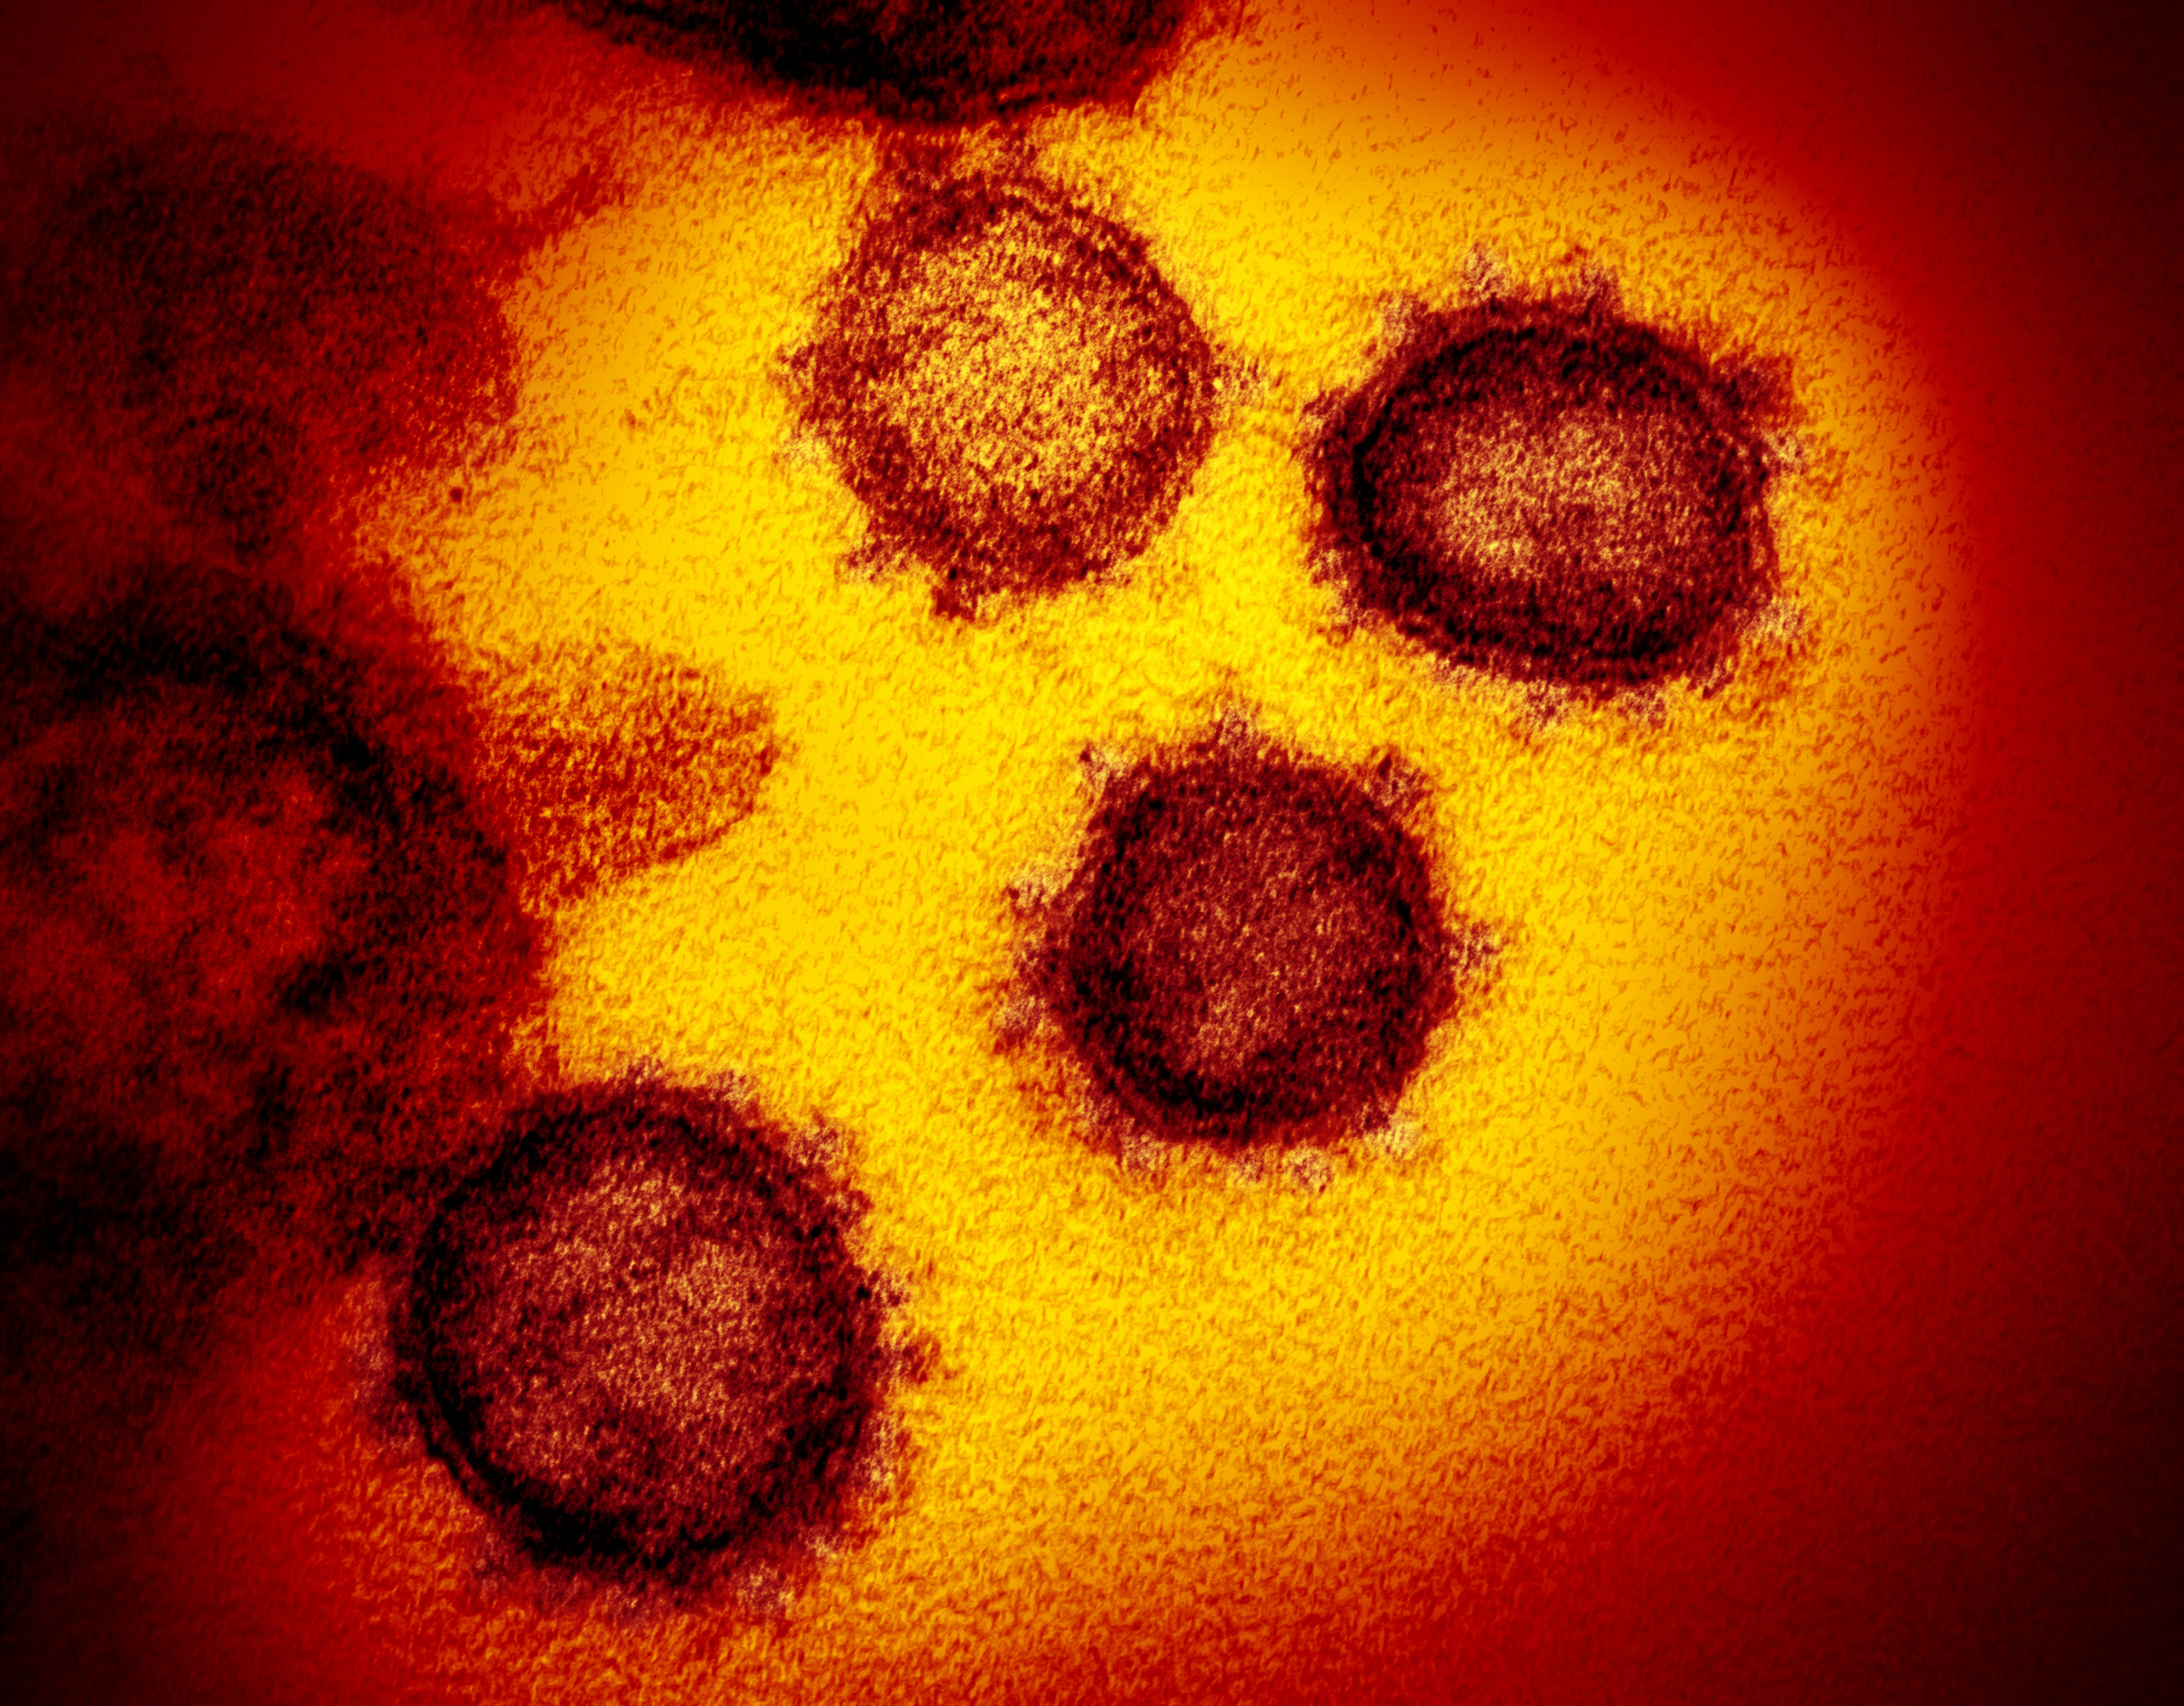
\includegraphics[width=.7\linewidth]{Figures/Coronavirus1.jpg}
  \caption{Transmission electron microscope (TEM) image of SARS-CoV-2—also known as 2019-nCoV, emerging from the surface of cells cultured}
  \label{fig:sub-first}
\end{subfigure}
\begin{subfigure}{.5\textwidth}
  \centering
  % include second image
  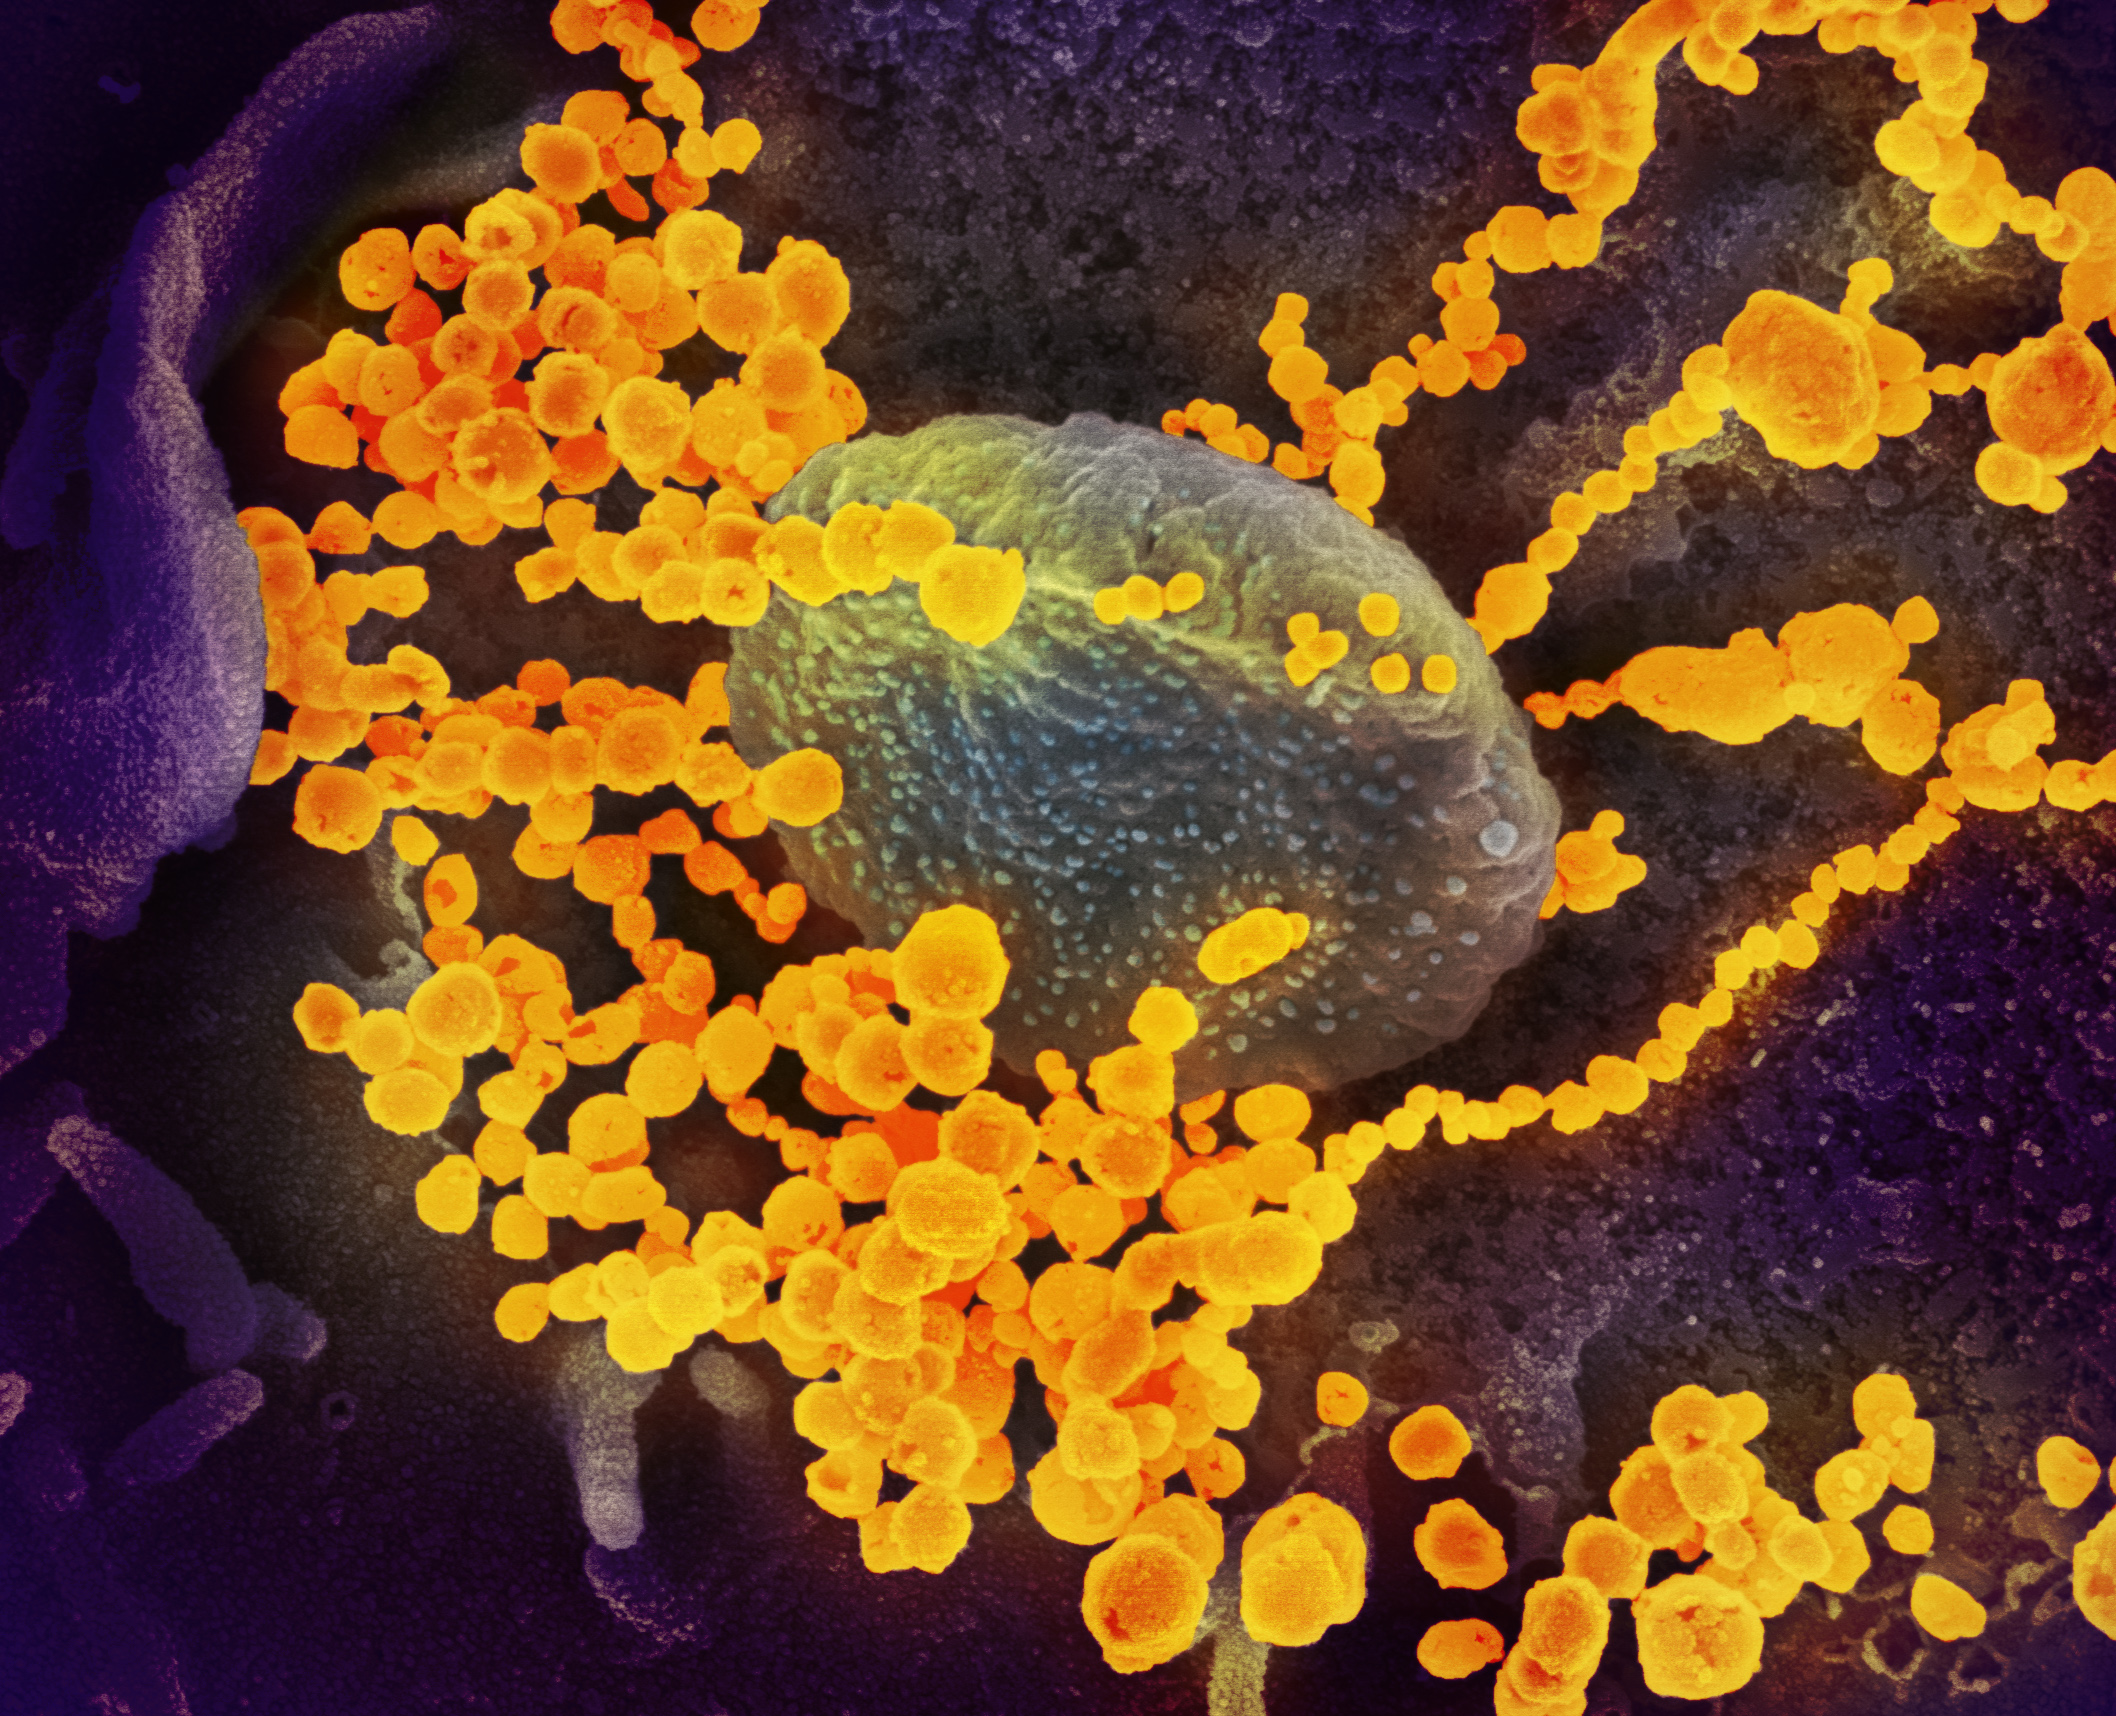
\includegraphics[width=.7\linewidth]{Figures/Coronavirus2.jpg} 
  \caption{Scanning electron microscope of the SARS-CoV-2 emerging from the surface of cells cultured}
  \label{fig:sub-second}
\end{subfigure}
\begin{subfigure}{.5\textwidth}
  \centering
  % include second image
  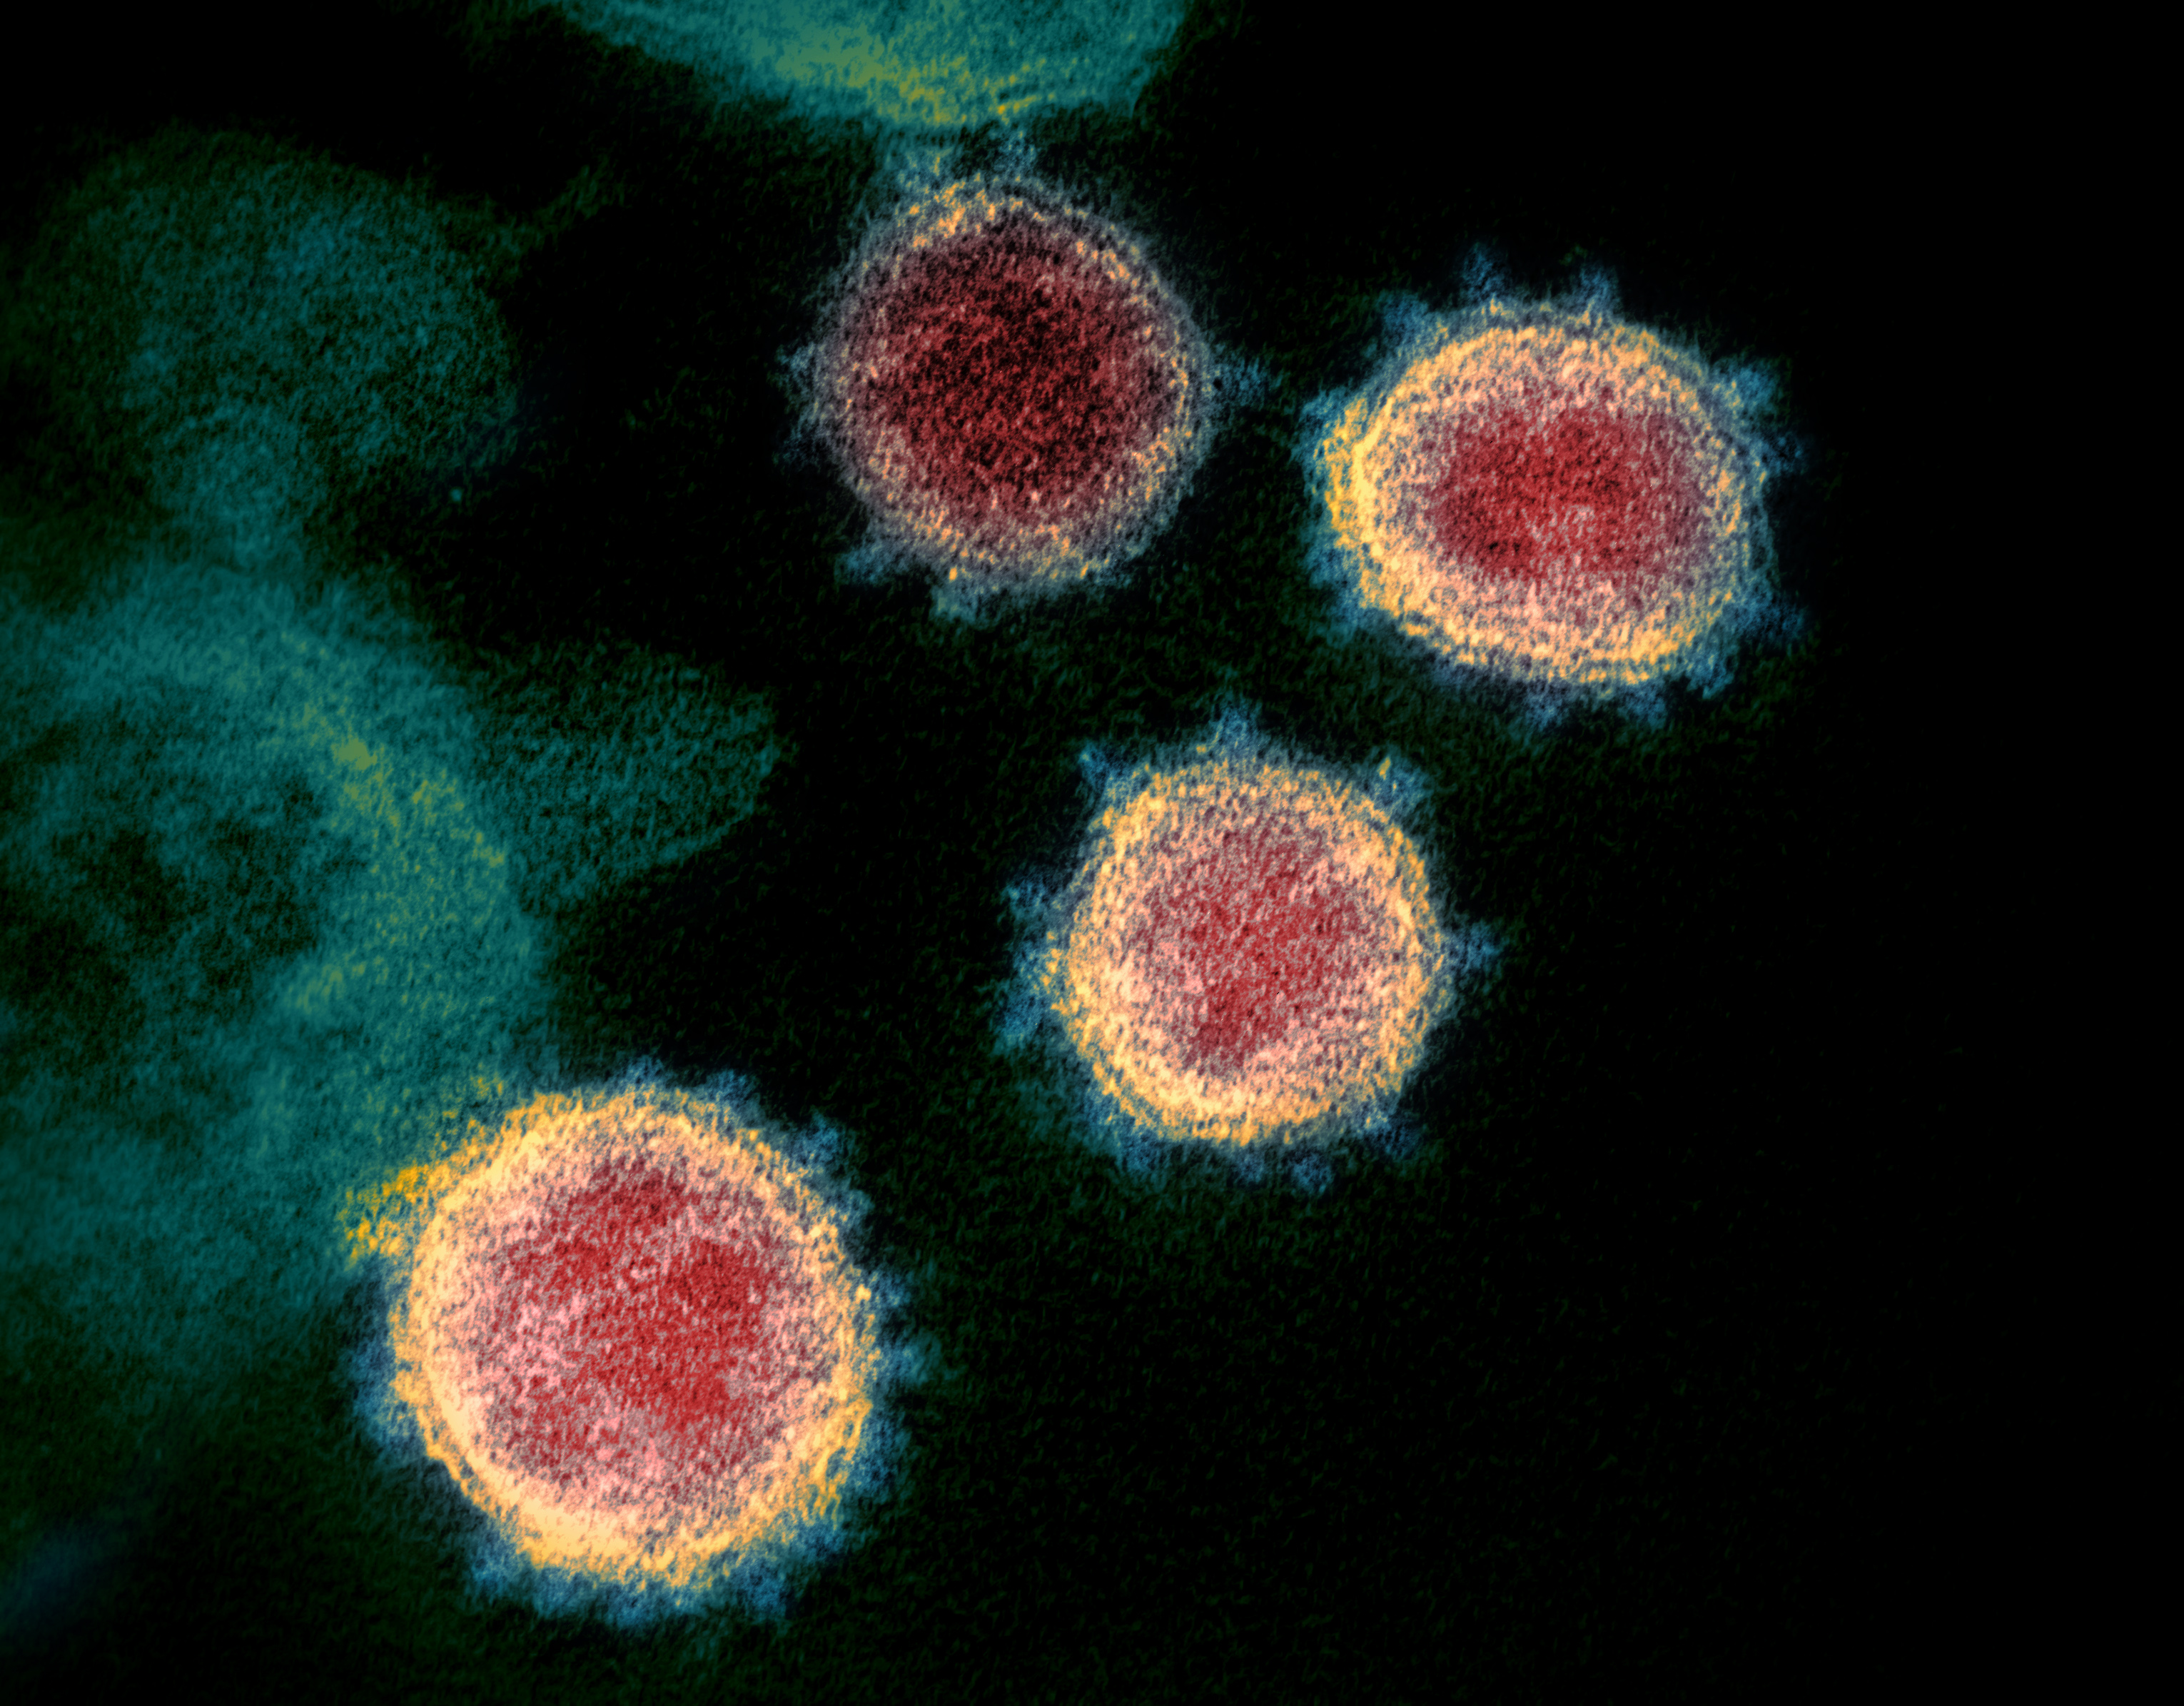
\includegraphics[width=.7\linewidth]{Figures/Coronavirus3.jpg} 
  \caption{TEM image of SARS-CoV-2. Not the spikes that gives the name coronavirus to the virus }
  \label{fig:sub-second}
\end{subfigure}
\begin{subfigure}{.5\textwidth}
  \centering
  % include second image
  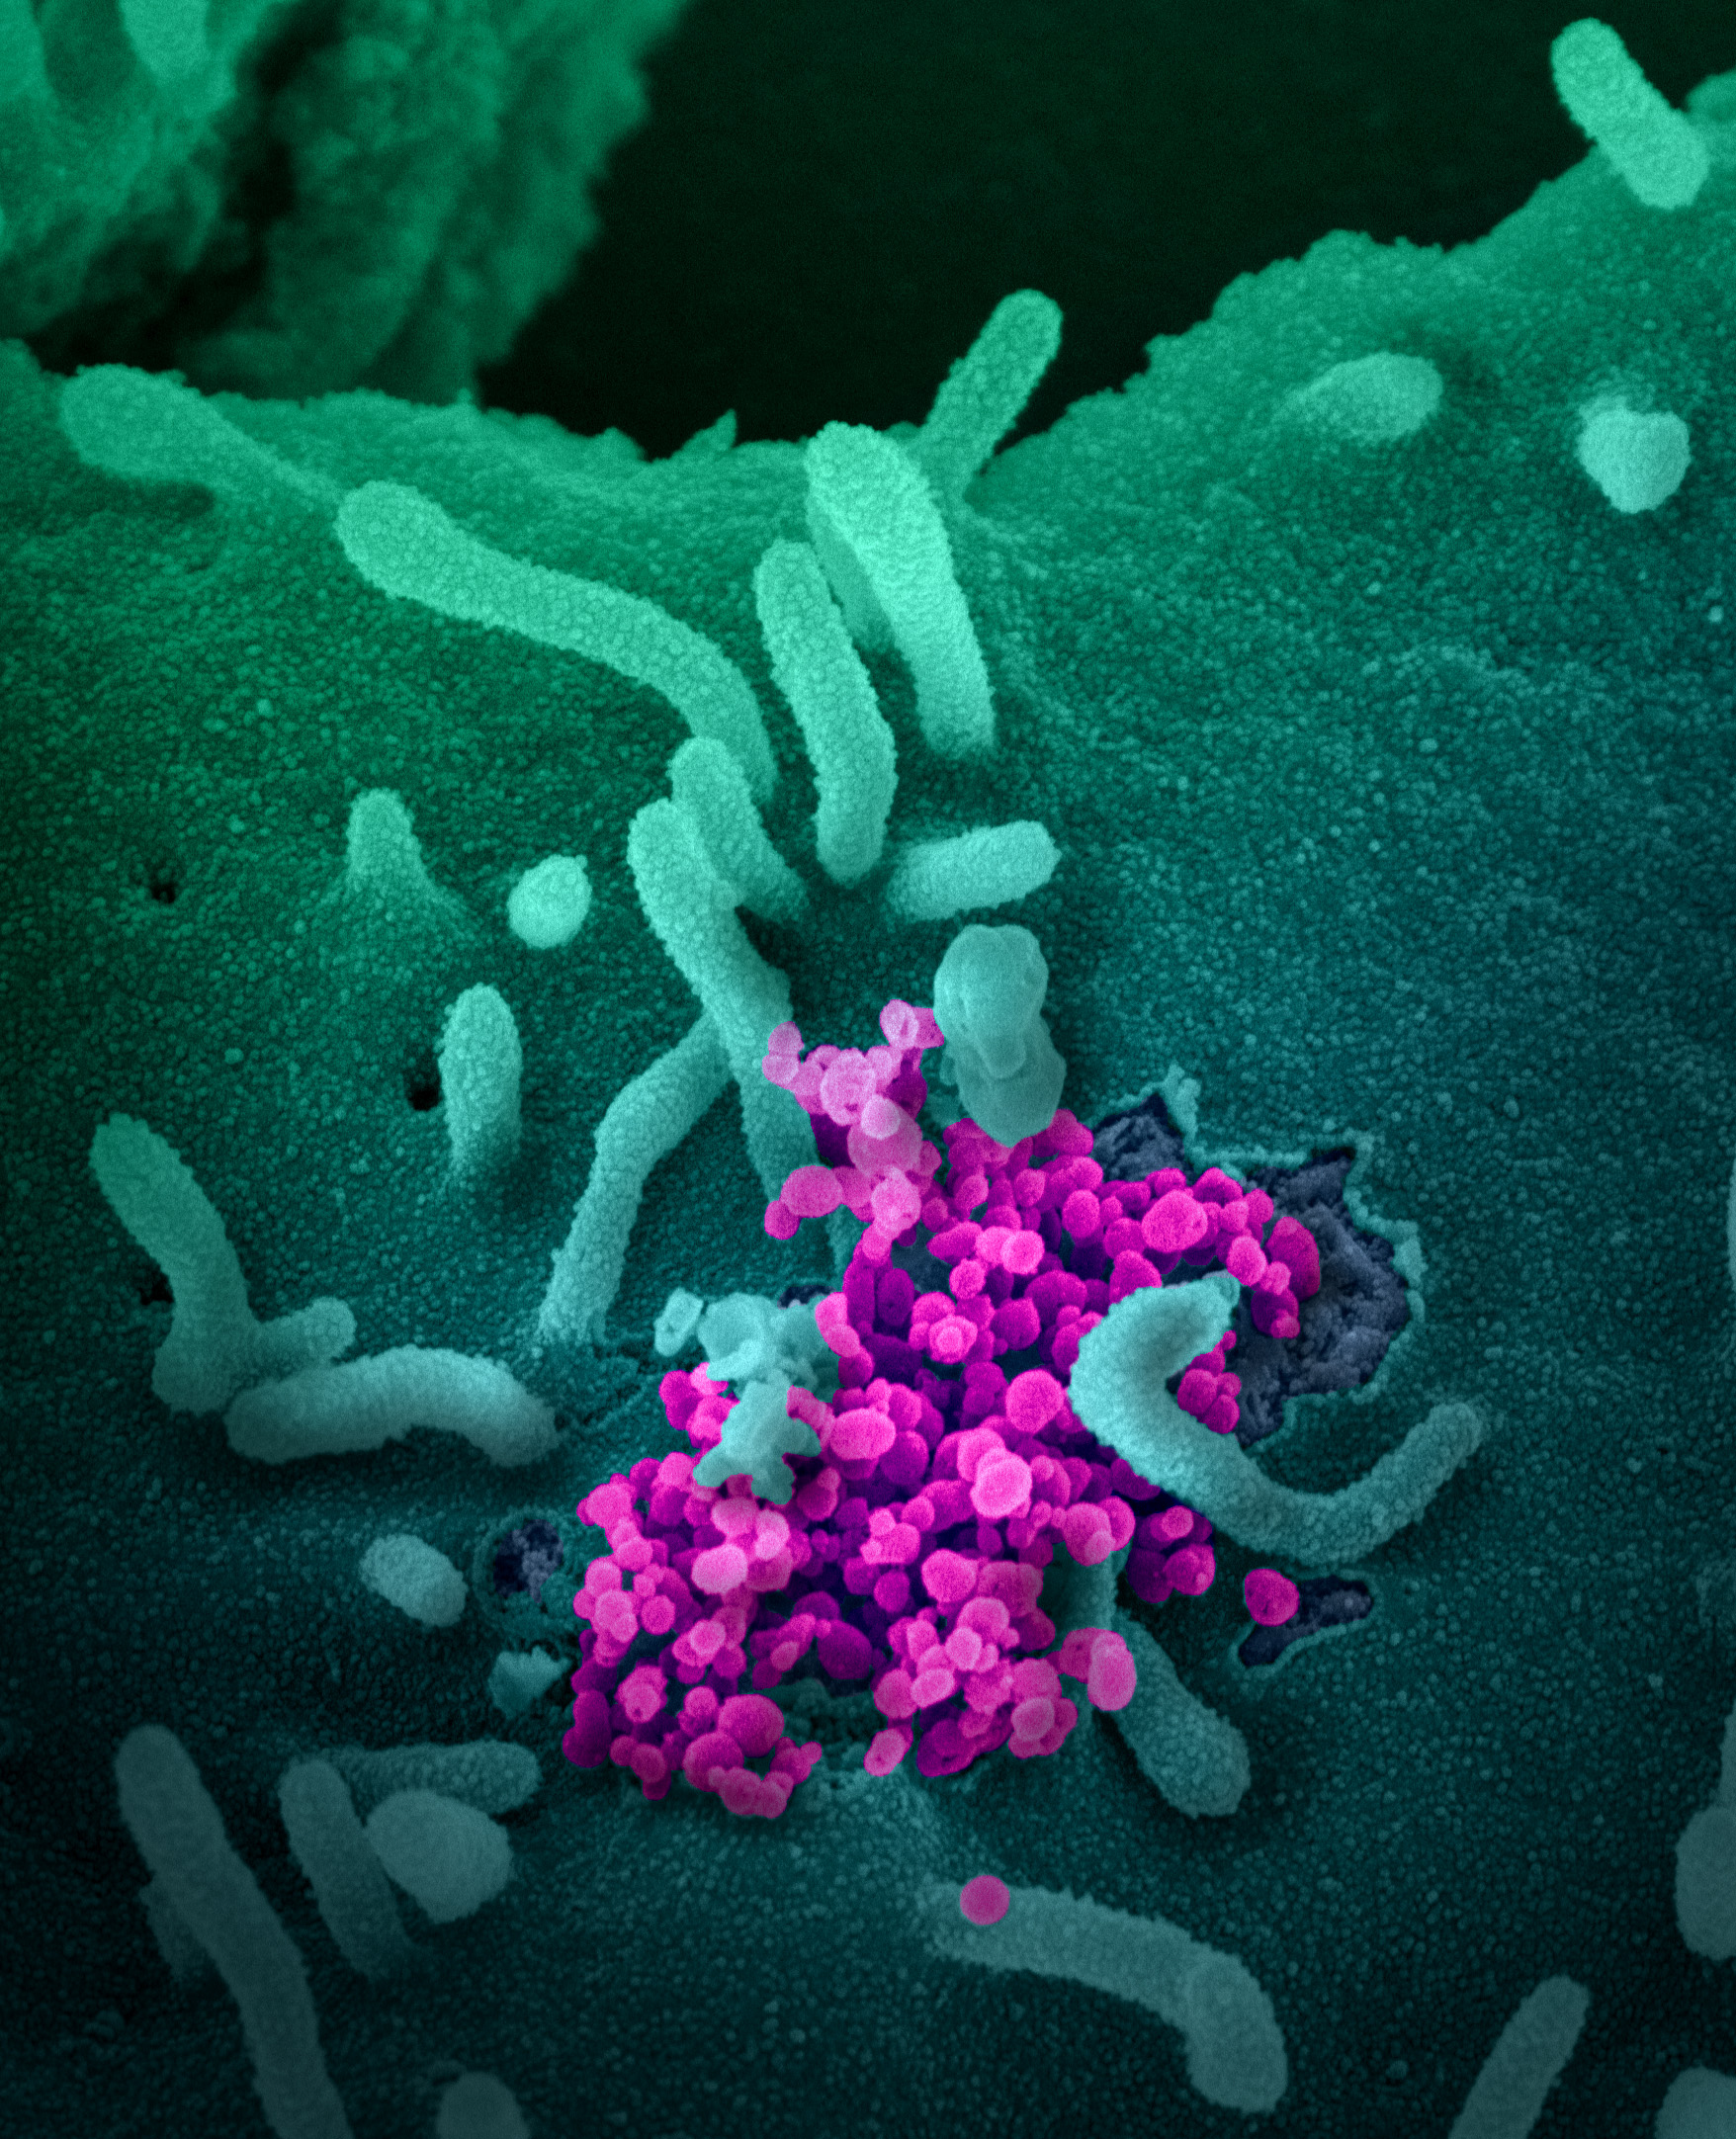
\includegraphics[width=.7\linewidth]{Figures/Coronavirus4.jpg} 
  \caption{SEM image of the virus}
  \label{fig:sub-second}
\end{subfigure}
\caption{Different pictures of the virus as reported by the NIAID’s Rocky Mountain Laboratories (RML) in Hamilton, Montana \cite{coronavirus+pictures}  }
\label{coronavirus_picture}
\end{figure}


In January the Chinese government imposed the quarantine for the city of Wuhan (almost 11M people); the quarantine was later expanded to the full province of Hubei (60M people) and then to the neighbour provinces Huanggang, Ezhou and Xianning. 
The virus then spread in Canada, Germany, Thailand and Japan and then in other different countries including Italy \cite{timeline+web}. In Italy the first cases, two Chinese tourist from Hubei, were reported in Rome \cite{corr+roma}; then  other cases were reported in Codogno (Lodi, Lombardy). Later the virus spread almost in all regions of Italy with a higher density in Lombardy, Veneto, Emilia-Romagna, Piemonte and Marche. Starting from 22nd of February, the Italian government started to impose the quarantine (red-zone) for eleven different municipalities, in particular Codogno, Casalpusterlengo, Lodi (included the neighbour municipalities) and Vo\textquotesingle. From this date onward, different restrictive measures were imposed starting from regions with the highest number of cases: public entrainment were almost suspended as well as schools and universities. Workers (in public and private sectors) were allowed, when possibile, to work at home (smart-working). Such measures culminated with a decree approved by the Italian government that divided Italy in three areas: the red zones, in which the municipalities with highest number of cases in which all the population was subjected to quarantine; the yellow zones (Lombardia, Veneto, Emilia Romagna) where schools, universities and public events, sports as well cinemas were suspended; the rest of Italy, in which no restrictive measures were adopted \cite{rep+dec1}; however 3 days later all schools and universities were suspended \cite{guard+01}. The restrictive measures were also extended up to all Italy with a further decree \cite{11marzo}. 

\subsection{Historical Background}



In the last centuries several cases of pandemic diseases were recorded: from our point of view, their dynamic is useful to understand and perhaps to model that further peaks may succeed the first one even with a highest death rate. 

\paragraph{The  deadliest pandemics in human history: the Spanish flu}

 The first one, which happens to be the biggest human pandemic (in terms of spread just as much as deaths \cite{potter2001history} ), is the Spanish Flu: this name is quite misleading since it was not originated in Spain, though the Spanish press was the first one to talk about it. Indeed, at that time (1917-1918) almost every other country was involved in the Great War and consequently the censorship was applied to the press . The origin of this disease is still under research: some scholars focused on the United States \cite{crosby_2003,barry2004site}, on France \cite{shanks2016no} and on Asia \cite{langford2005did}.  The disease was ascribed to the virus A/H1N1, a subtype of influenza A Virus. The spread of the disease was strongly amplified by the fact that many people lived in very bad hygienic conditions. As one can see from Fig.\ref{SpanishFLU} there were basically three waves: the initial spread, the second wave and the third wave. The second wave, that was the most lethal one, coincides with the end of the war and with the coming back of the troops: the close contact inside the trains, and the diffusion of the troops inside their home villages/cities increased abruptly the contagion rate and then the death rate. Furthermore, this effect was amplified by the fact that a more deadly mutation of the virus became widespread \cite{barry2008cross}. As pointed out by different scholars, such effect was enhanced by the fact thst sick people, which infection potential was higher, were transferred by train to the hospitals. Immediately, the virus spread with a higher rate \cite{wever2014death}. As it is possible to note from Fig. \ref{Mortality_spanish_flu} this second wave was largely more deadly for young people with respect the first wave. Finally, looking at plot \ref{SpanishFLU}, a third wave also manifested itself in the beginning of 1919: here, the mortality was higher with respect to the first one, but lower to the second one. In the end, this pandemic infected 500 million people and killed something between 17 and 50 million \cite{spreeuwenberg2018reassessing}. It is worth nothing that, just to compare, the casualties in the Great War were from 8.8 to 10.7 million among soldiers and 11 million among civilian \cite{haythornthwaite1996world}


\begin{figure}[h]
 \centering
 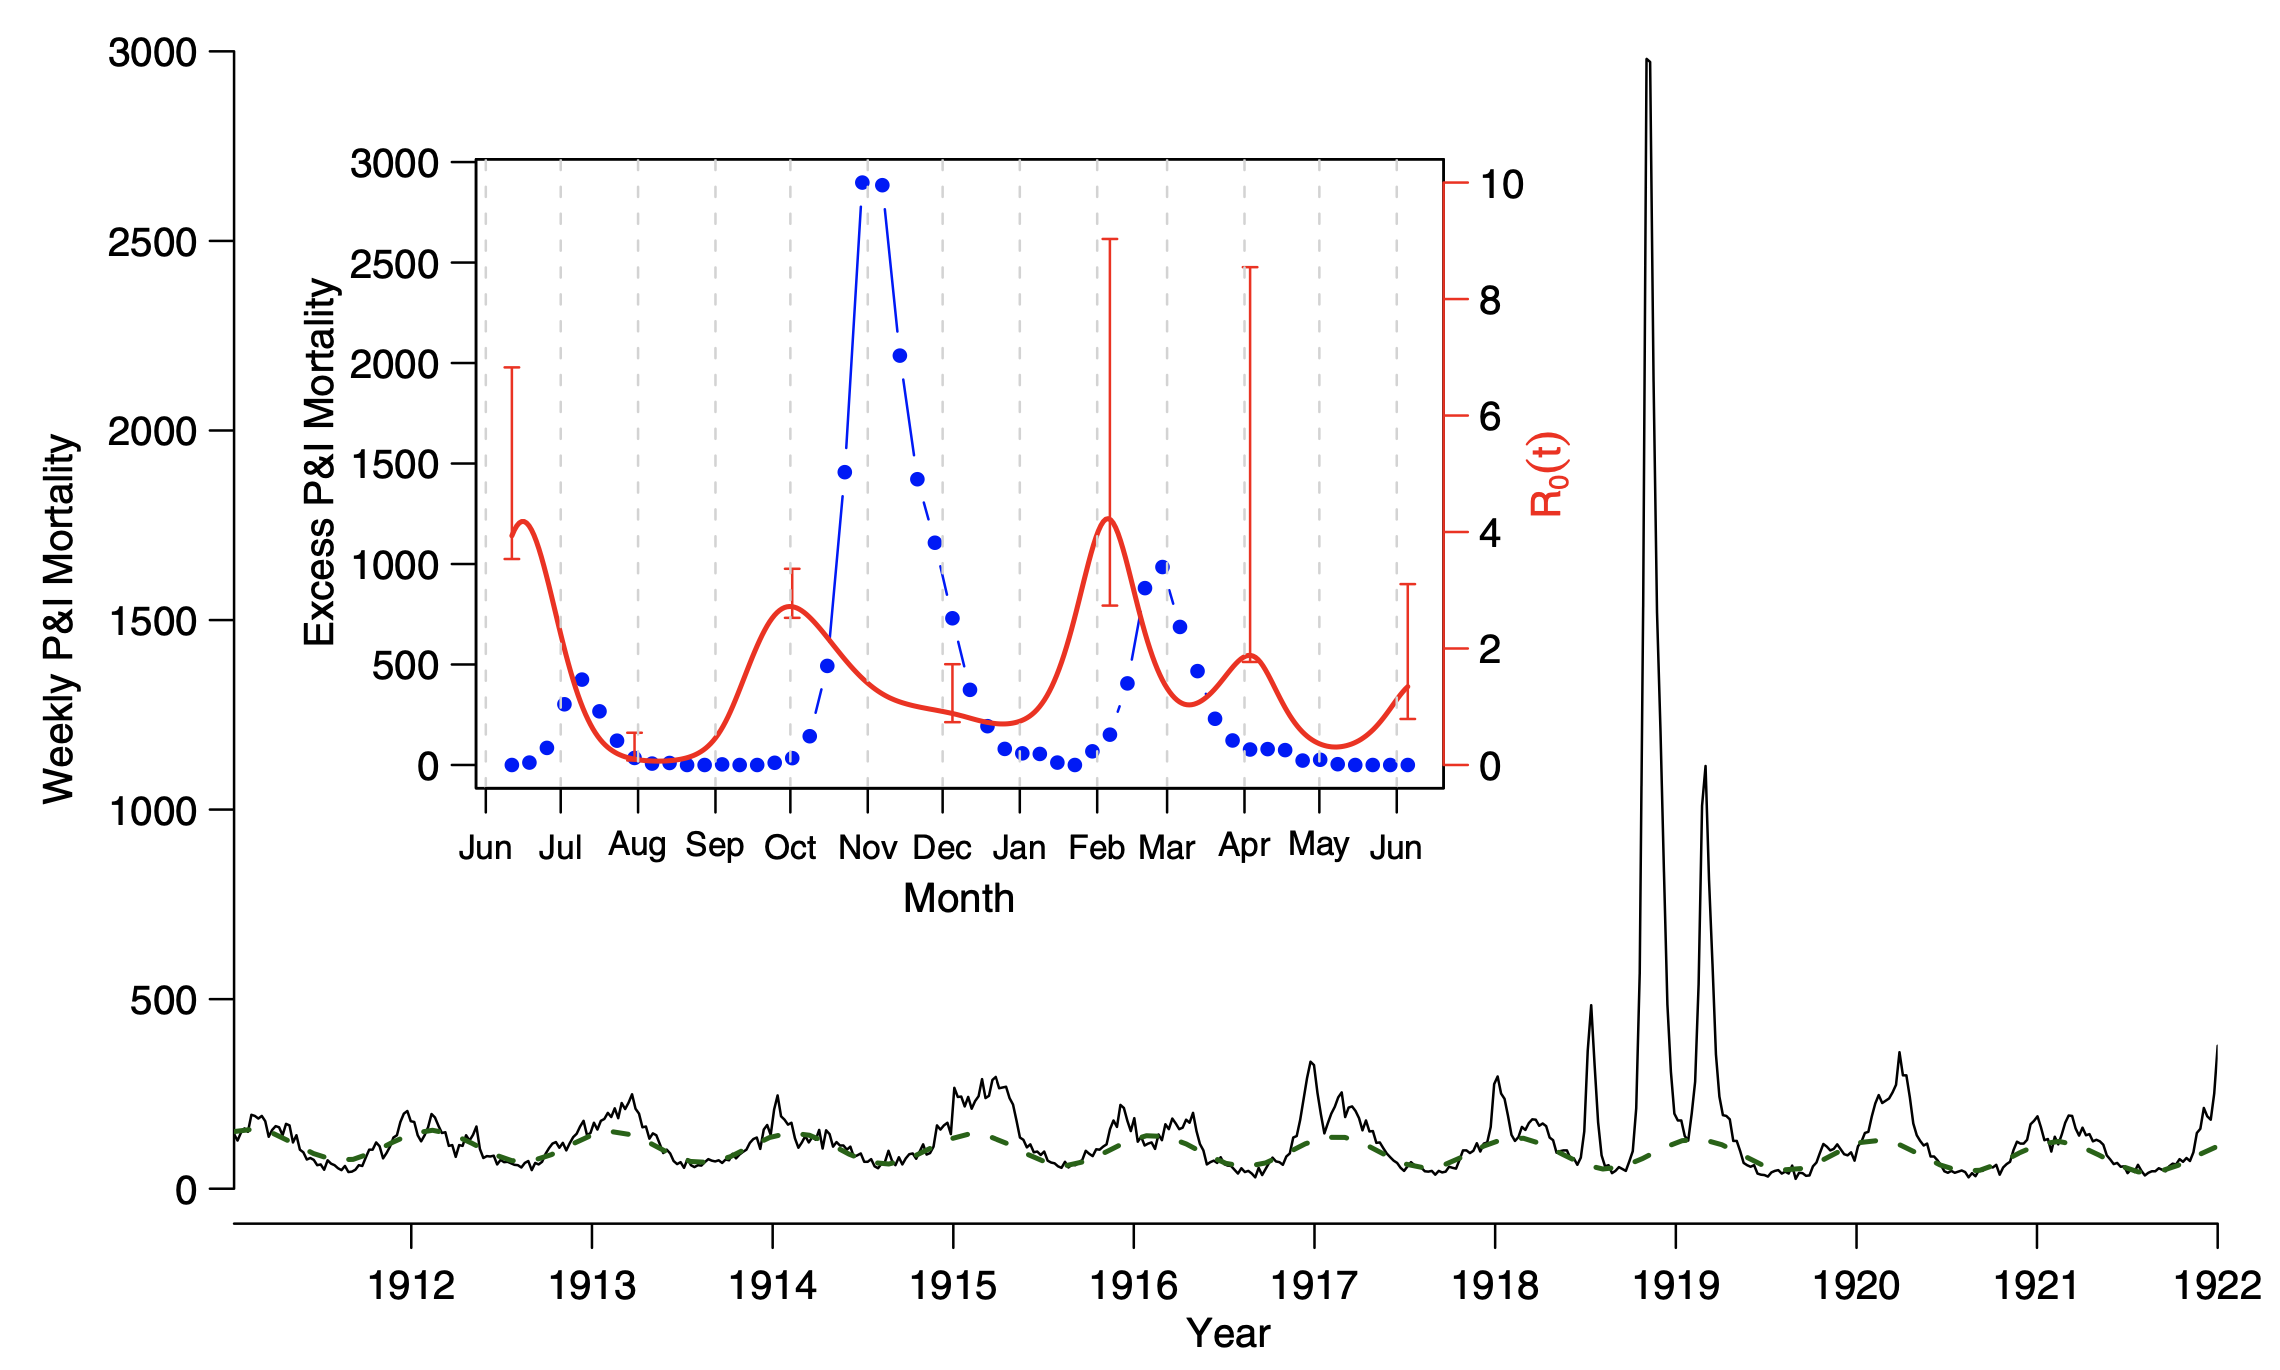
\includegraphics[width=1\linewidth]{Figures/SpanishFLU.png} 
 \caption{Pneumonia and Influenza mortality from 1910-1922 in London: note the three peaks due to the spanish flu. The variation of the diffusion rate R$_{0}$ is reported in the box. Image source: Ref. \cite{he2011mechanistic} }
 \label{SpanishFLU}
\end{figure}

\begin{figure}[h]
 \centering
 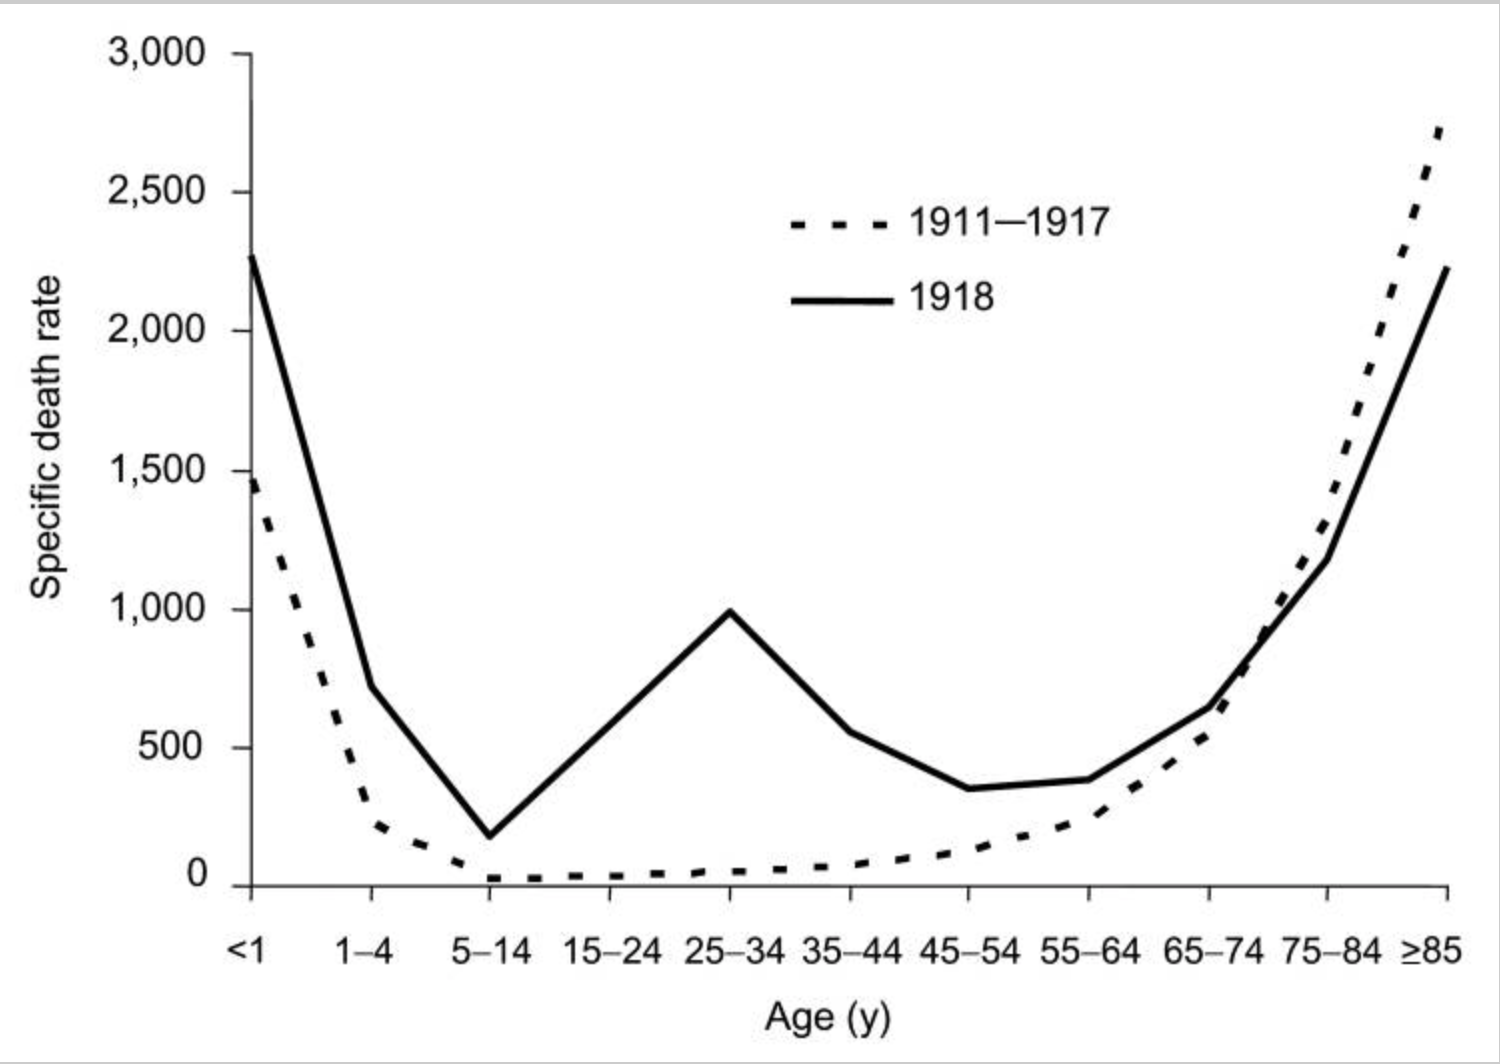
\includegraphics[width=0.6\linewidth]{Figures/Mortality_spanish_flu.png} 
 \caption{Mortality range distribution for the two waves of Spanish flu: note that the second one was more severe for the young people. Image source: Ref. \cite{taubenberger20061918}}
 \label{Mortality_spanish_flu}
\end{figure}

\clearpage

\paragraph{The Asian Influenza (H2N2)}

In 1957 different cases another virus of influenza ( A/H2N2 ) spread in China starting from Guizhou \cite{strahan1994oriental} . In this case, at difference with respect to the Spanish flu, the scholars were able to isolate the virus (the virus of the former was only isolated in 1933). It was proposed that the virus may be originated from mixing of avian and human influenza (see Fig. \ref{Mixing_Flu}). The virus diffused in Hong Kong in April then in Singapore, Taiwan and Japan and then globally \cite{saunders2016reviewing} . While for the US a crucial role for the spread was supposed to be played by naval  bases \cite{henderson2016development,saunders2016reviewing}, for Europe the same role was played by the  land route trough Asia \cite{langmuir1961epidemiology,saunders2016reviewing}. Scholar also pointed out the role of a church conference in Iowa \cite{payne1958some} were almost 1600 people from all countries met. Furthermore the open of school in fall increased abruptly the spread of the virus (40-60 \% clinical attack rate) \cite{henderson2009public,saunders2016reviewing}. Also in this case it was reported a second wave (or perhaps others one, see Fig. \ref{Asiatic_HK_flu}) more lethal than the first one \cite{ebasianflu} . In this case, contrarily to the Spanish Flu a vaccine was developed although \cite{henderson2009public}, it was argued that its diffusion was not effective to diminish the effect of the pandemics \cite{jensen1958influenza}. It was nothing that according to scholars \cite{trotter1959asian} no effective measures of quarantine or other non-pharmacological one were undertaken by the authorities \cite{trotter1959asian} due to the mild symptoms \cite{saunders2016reviewing}. The total toll for this pandemic was from 1 to 1.4 million deaths according to the WHO \cite{who_influenza}: from our point of view this pandemic is a counterfactual teaching lesson about what happens when a pandemics is underestimated (and so no restrictive measure is taken)  due to its relative  mild synthoms 

\begin{figure}[h]
 \centering
 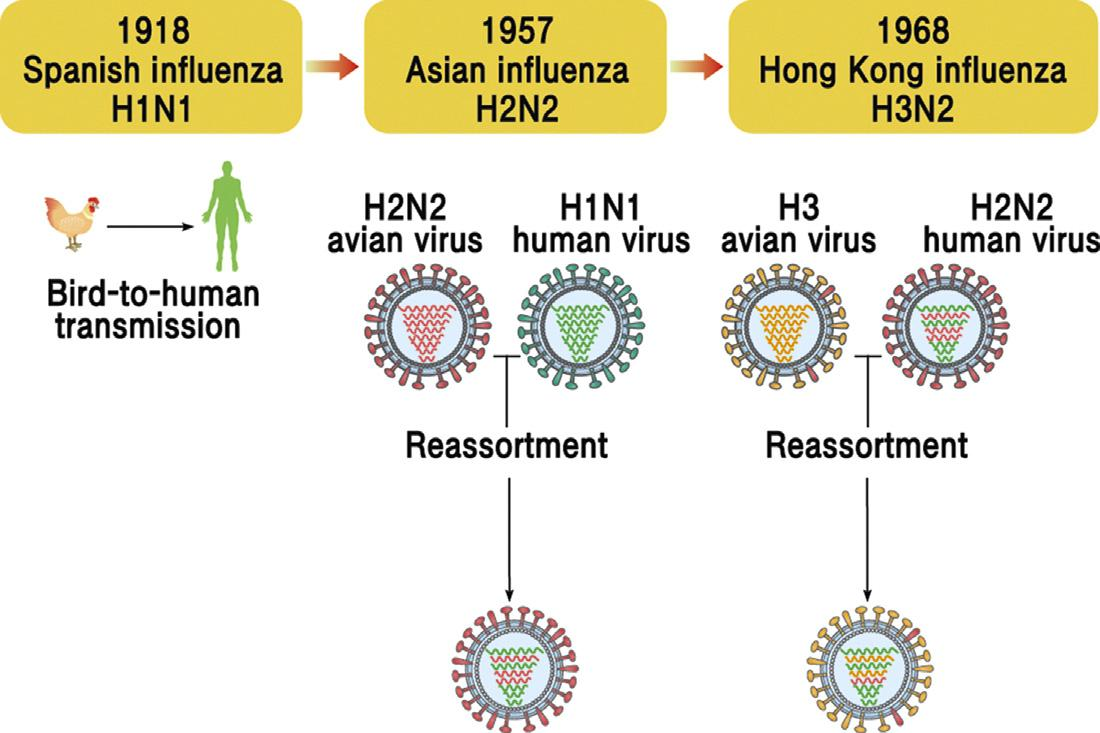
\includegraphics[width=0.8\linewidth]{Figures/Mixing_Flu.jpg} 
 \caption{Wang-ShickRyu diagram for the explanation of the Spanish, Asian flu and Honk-Kong flu .  Image source: Ref.  \cite{RYU2017195}}
 \label{Mixing_Flu}
\end{figure}

\begin{figure}[h]
 \centering
 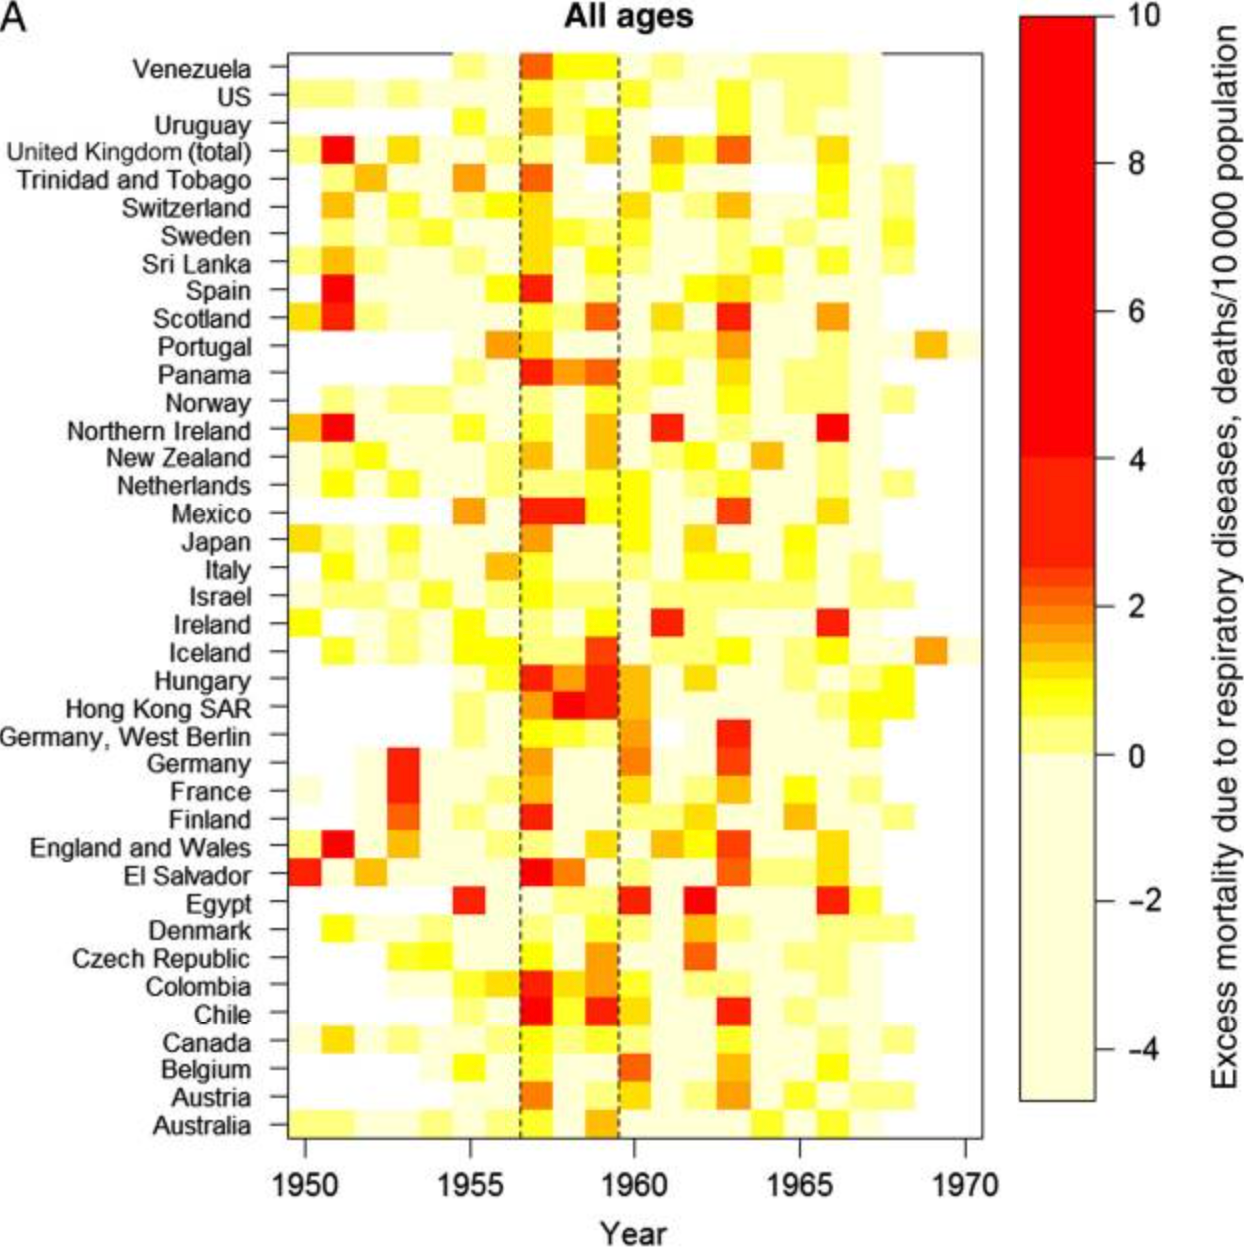
\includegraphics[width=1\linewidth]{Figures/Asiatic_HK_flu.png} 
 \caption{ Excess mortality due to respiratory disease from 1950 to 1970 as reported by Viboud et al. The dashed lines marks the timing of the Hong Kong flue. Image source: Ref.  \cite{viboud2016global}}
 \label{Asiatic_HK_flu}
\end{figure}


\clearpage


\paragraph{Motivation} \label{Motivation}
In order to have a thorough insight of the spread of the COVID-19 disease and its effects on italian population, we propose a ShinyApp, called disCOVIDer19, that gathers, presents and analyzes the numbers of new and cumulative infections, hospitalized and intensive care patients, deaths and recoveries, over the whole country and over its individual regions and provinces. A detailed guide to the functioning of the App is available in sections \ref{Data Origin} and \ref{Panels}. As regards the analysis panel, we fitted the cumulative cases with a logistic curve, in order to get a bird-of-eye view on the general and specific trends as well as on the effectiveness of the restrictive measures imposed by the Italian government. The theoretical foundations of this fit and how to manage and use it will be discussed in the section \ref{Theoretical Background} and \ref{sub:Data Analysis}. Beside the logistic curve, we also considered a statistical approach, largely diffused among economists, that considers the number of total cases in each day as a time series: on this basis we were able to make use of a particular tool, which will be briefly introduced in the section \ref{Theoretical Background}, that allowed us to make a further forecast about future cases. This latter becomes useful in case of large deviations from logistic distribution.
Finally, we must remark that our approach is informational: we do limit ourselves to list and comment our findings without claiming rather delicate conclusions, expecially about predictions, which many people hinge on nowadays and many lives too, unfortunately.
 
%----------------------------------------------------------------------------------------
%	METHODS
%----------------------------------------------------------------------------------------

\section{Theoretical Background} \label{Theoretical Background}
Several models were proposed in the literature for modelling the spread of a disease \cite{keeling2011modeling}: here, we are going to consider a relative simple model taken from the growth dynamics of populations.

\subsection{Population growth dynamics}
The dynamics of population was founded by Thomas Malthus in 1817 \cite{malthus1817essay} with his well known equation: 

\begin{equation}
x_{n+1}=x_{n}(1+r)
\end{equation}

where $x_{n}$ stands for the population at time and $r$ the growth rate. Renaming $x$ to $P$ and applying recursive substitution, we get: 

\begin{equation}
P_{n+1}=P_{0}(1+r)^{n+1}
\end{equation}

in which $P_{0}$ represents the initial population. This discrete model can be reshaped in to a continuous one in the following way: 

\begin{equation}
\dot{P}(t)=rP(t)
\end{equation}

That's a first order ODE with separable variable. Integrating yields:

\begin{equation}
P(t)=P_{0}e^{rt}
\end{equation}

Malthus, of course, did not believe that the population could grow ad infinitum with an exponential trend and, since he estimated that the resources growth follows a linear path, he argued that, at the intersection of the two curves, a consistent part of the population will not have access to the resources. Thus he expected that the exponential growth realizes only in the first part of the growth. Basing on these arguments, in 1838 Belgian mathematician Pierre-François Verhulst developed a model \cite{verhulst1838notice} whose new feature and key point was the maximum size of the population allowed by resources, that is the natural upper limit of coexisting individuals in a particular environment, usually called the \emph{carrying capacity}, here indicated as $K$ ($P$ and $r$ have the same meaning of the previous model):

\begin{equation}
\dot{P}=rP\left(1-\dfrac{P}{K} \right)
\end{equation}

that has the following analytic solution: 

\begin{equation}
P=\dfrac{KP_{0}e^{rt}}{K+P_{0}(e^{rt}-1)}
\label{logistic_equation}
\end{equation}

In Fig.\ref{Malthusian_growth_vs_logistic_growth} this solution is compared to the Malthusian one: as one can see, the logistic growth shows a saturation effect towards the asymptote of carrying capacity. This completes Malthus's intuition, as it represents population growth before and after the intersection between the linear resources curve and the natural exponential growth. It is worth noting that  in a neighbourhood of the origin the two curves are identical; later, the logistic curve bends down, still increasing, till it reaches the saturation region, in which it becomes almost flat. 

\begin{figure}
 \centering
 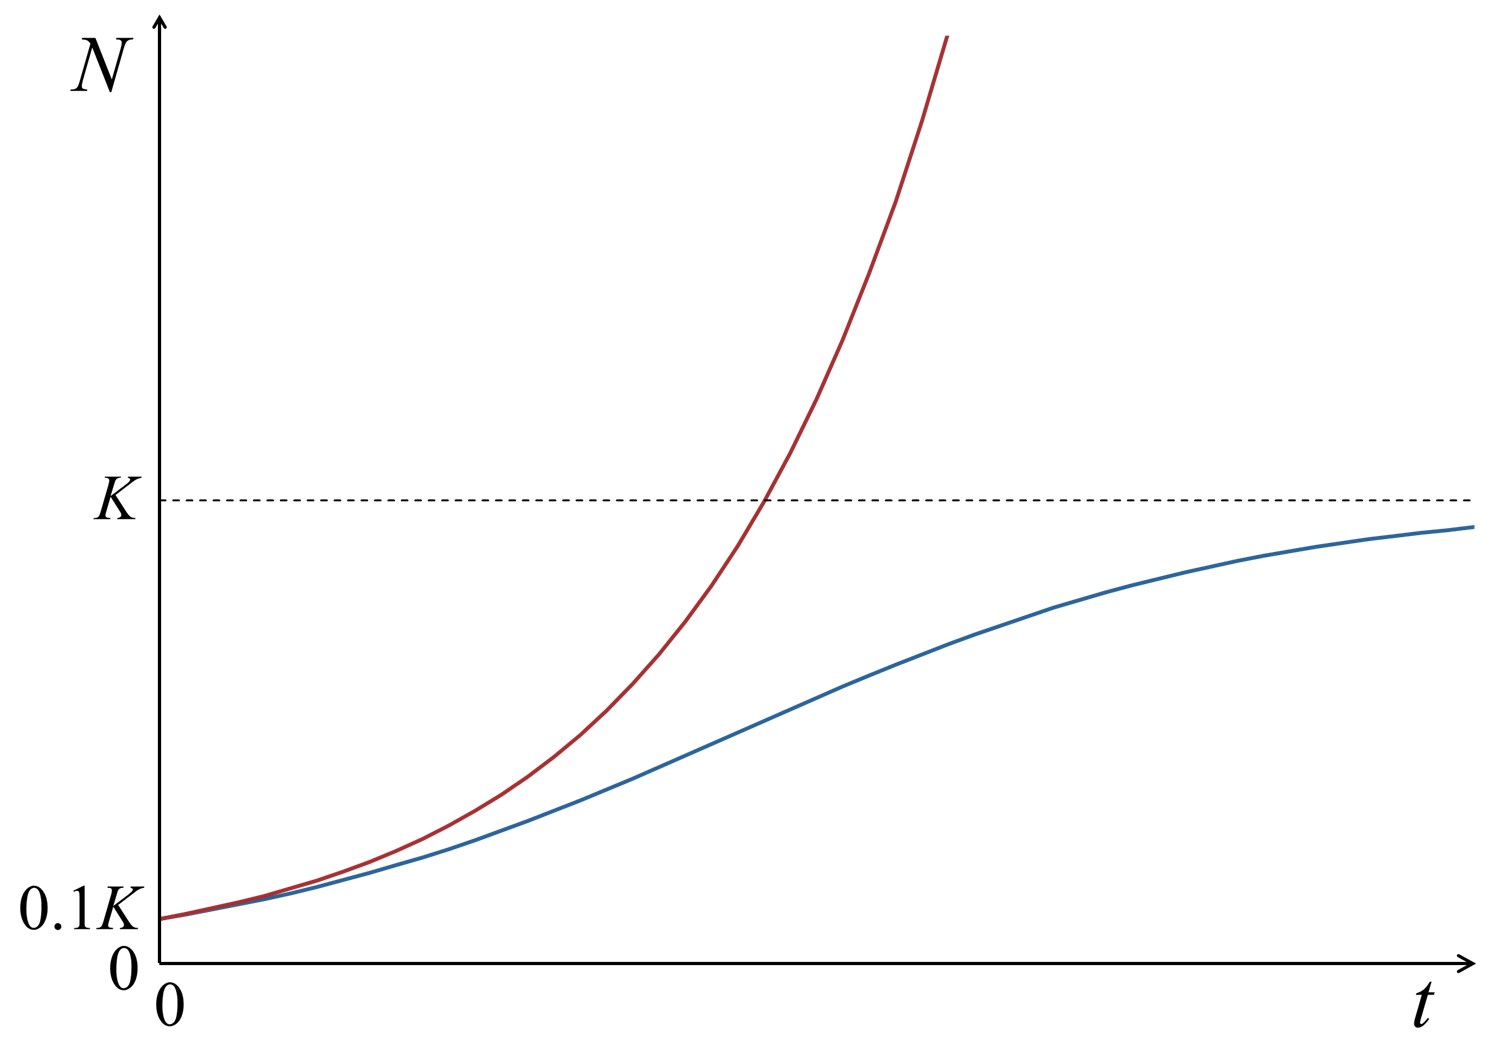
\includegraphics[width=0.8\linewidth]{Figures/Malthusian_growth_vs_logistic_growth-2.jpg} 
 \caption{The Malthusian growth (red line) compared to the logistic growth (blue line). The carrying capacity is marked with a black dashed line. Image taken from \cite{malthus_vs_logistic}}
 \label{Malthusian_growth_vs_logistic_growth}
\end{figure}

\subsection{Application to the epidemiology}

The dynamics of the model described before can be used to shape the spread of an infection  \cite{serfling1952historical,ma2014estimating}. In this case the population $P$ is replaced with the total number of infected people, $P_{0}$ with the number of initially infected people, $r$ with the spreading rate and the carrying capacity $K$ with the maximum number of people that can be infected. The latter is the key point for the modelling: in principle, this parameter would be equal to the population number; in practice, due to restrictive measures and, possibly, vaccines, a large share of the total population won't enter the computation, thus lowering the carrying capacity. So, we can argue that the effectiveness of the restrictive measures can be inferred from the behaviour of the cumulative curve (except, of course, if the number of infected people is close to the population size). It is worth noting that, for each non-quarantined infected, the carrying capacity is increased up according to the individuals that can be infected by these subjects. If this contribution is not negligible a new logistic growth may be found, with of course an exponential starting behaviour. Thus the prediction with the logistic curve should be taken as an evaluation of the impact of restrictive measures and as the \emph{best scenario} that may occur. For this reason it is advisable to see the logistic curve as a local (in time) estimator. 
In fact, one can model a differential set of equation were the carrying capacity is time dependent. This possibility may be considered  by the authors in a future version of this App. Furthermore, we remind that other similar models such as Gopertz, Richards or Bertalanffy can be used to shape the COVID-19 outbreak\cite{ma2014estimating}: the authors may consider to include them in a future version of this App.



\subsection{Time series approach}

\subsection{An ab-initio approach: the SEIR model}

%------------------------------------------------

\section{Data Origin} \label{Data Origin}



%------------------------------------------------

\clearpage

\section{Panels} \label{Panels}

\subsection{Home}

The home panel provides an overview of the COVID19 spread in Italy. The data shown are synchronised with the civil protection database. Whenever the App is started, a check for the updates is performed and their occurrence is indicated in the \textit{most recent updates }section. The home panel consists of two main sections: the choropleth map and the summary statistics. The choropleth map (Fig. \ref{Home_fig1}) is an interactive heat map with breakouts by region and by province tracking the number of Covid-19 cases. 

\begin{figure}[h]
 \centering
 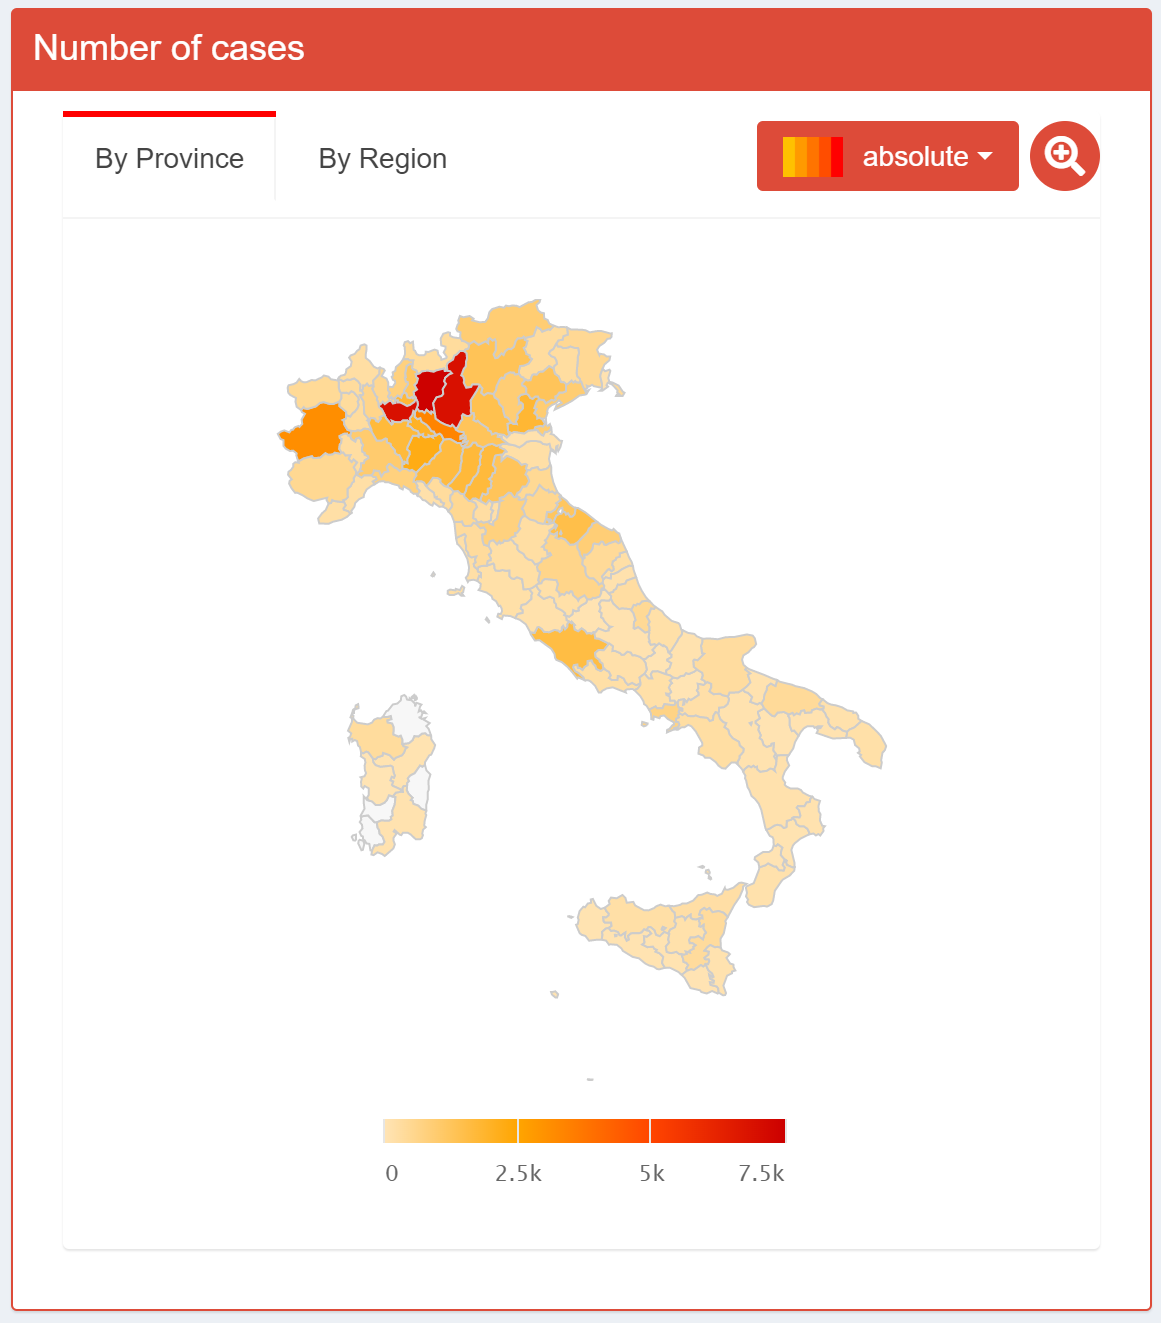
\includegraphics[width=0.5\linewidth]{Figures/Home_figure_1.png} 
 \caption{Choropleth map by province showing absolute number of Covid-19 cases}
 \label{Home_fig1}
\end{figure}

Beyond the raw absolute number of total cases by province/region we propose two other indicators which introduce some form of normalisation to improve the comparability of the different geographical areas. These indicators are percentage and density (Fig. \ref{Home_fig2}).

\begin{figure}[h]
 \centering
 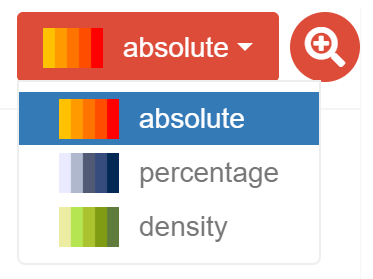
\includegraphics[width=0.5\linewidth]{Figures/Home_figure_2.png} 
 \caption{Input selector where the user can choose the three different breakouts absolute, percentage, and density}
 \label{Home_fig2}
\end{figure}

The percentage indicator is calculated dividing the total number of COVID19 cases by the population of the respective region/province (the latter retrieved from Istat \cite{Istat+res0,Istat+res1}).
\begin{equation}
percentage~cases = \frac{total~cases}{local~population} \times 100
\end{equation}
This indicator ensures that the number of cases in more populated areas are not over-indexed compared to less populated ones. Similarly, it ensures less populated areas are not under-indexed. 
The density indicator accounts for the territorial extension (in $km^2$) of regions/provinces expressed in parts per thousand (\textperthousand ) and is calculated as follows:
\begin{equation}
density~cases =  \dfrac{total~cases}{territorial~extension}\times 1000
\end{equation}
This indicator combines the population density with infection spread, offering a control over space. Indeed, it is directly proportional to population density and to percentage cases:
\begin{equation}
\begin{split}
density~cases & =   \dfrac{total~cases}{local~population} \cdot \dfrac{local~population}{territorial~extension} \times 1000 \\  & = percentage~cases \cdot density~population \times 1000
\end{split}
\end{equation}
It is enhanced by densely populated territories, which, by the way, may in turn enhance spread infection too.
Finally, the summary statistics section (Fig. \ref{Home_fig3}) provides some barometer level statistics regarding the current total number of COVID19 cases in Italy with three further breakouts: intensive care, hospitalised, and home isolation.

\begin{figure}[h]
 \centering
 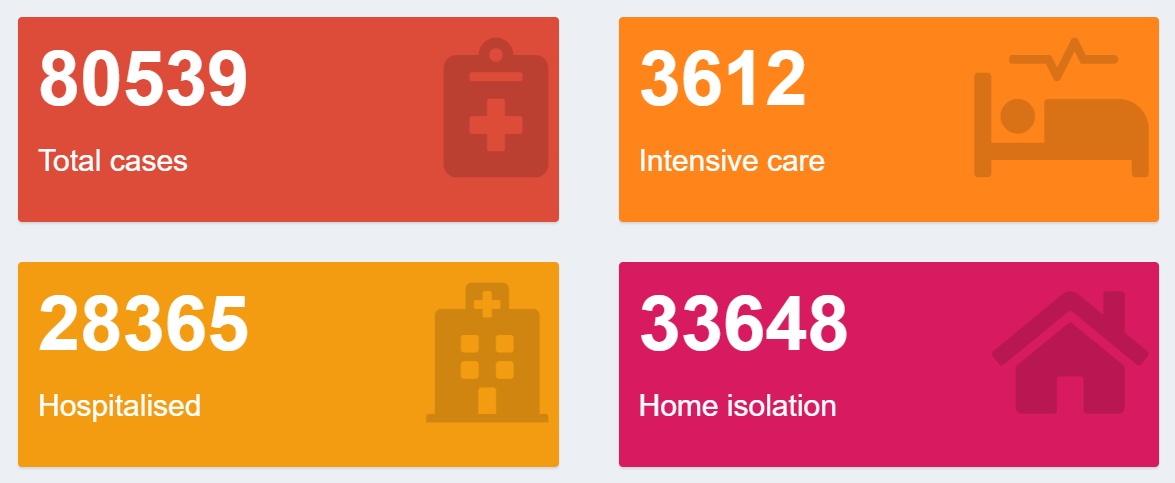
\includegraphics[width=0.5\linewidth]{Figures/Home_figure_3.png} 
 \caption{Boxes with syncronised barometer level statistic about the Coronavirus}
 \label{Home_fig3}
\end{figure}


\subsection{Data Inspection}\label{Data Inspection}

The \textit{Data Inspection} panel provides an exploratory analysis of the COVID19 spread in Italy and it consists of 2 main sections: an introductory inspection followed by a deeper inspection.

The first section introduces the user to a higher-level time series with the daily frequency of the number of Covid-19 cases broken down into symptomatic, recovered, deaths, and intensive care (Fig. \ref{fig:Inspection_general_info} in the \textit{General info} box). The cumulative cases add up each day while the daily cases are obtained by taking the first difference of the cumulative series ( $y_t - y_{t-1}$ ). When these time series capture all the stages of the pandemic evolution, the daily data are expected to assume a bell-shaped curve with a peak while the cumulative series a shape that is more similar to a logistic curve. The user can select different options spanning from the macro-level country view to the more granular province-level. In the same \textit{General Info Box}, the second tab provides direct access to the raw data (Fig. \ref{fig:Inspection_rawdata}) which is behind most of the visualisation used in the \textit{Home} and \textit{Inspection} sections of the dashboard. Through some input selectors and buttons, the dataset can be queried to show the information that is of most interest for the user.
The \textit{Infected Age Distribution} box 

The next chart shows the age distribution of infected patients (Fig. \ref{fig:Age_distribution}) with a region selector that offers the possibility to further investigate local-level dynamics and spot regional differences. The data was retrieved from Istituto Superiore di Sanità (ISS) \cite{epicentro} which is the National Institute of health in Italy. The information dates back to the 30$^{th}$ of March 2020. The chart shows the age distribution of the population which is divided into 10 age bins each one representing a 10-year interval. In particular, the bar chart indicates the absolute number of infected people in the respective age category while the pie chart shows the percentage breakdown of cases.

The \textit{Deeper Inspection } section consists of 4 different types of visualisations. The first two are located in the two tabs of the box called \textit{Intensive Care Information}. As the title suggests, these charts provide a comparative visualisation across regions of intensive care occupancy in hospitals. While one chart shows the occupancy/capacity index in percentage terms (Fig. \ref{fig:Inspection_perc_occupancy}), the other shows absolute figures of capacity and occupancy by region (Fig. \ref{fig:Inspection_occupancy2}). In particular, the occupancy index is calculated by dividing the percentage occupancy in the selected day by the hospital initial intensive care capacity at the start of the pandemic.

\begin{equation}
percentage~occupancy = \dfrac{occupancy}{capacity} \times 100
\end{equation}
It is worth noting that occupancy may be higher than the total number of available spots due to the fact that the beds in intensive care may have been more recently upgraded (see Sec. \ref{Data Origin}). The date selector, allows the user to explore the time evolution and variations of such quantities. The third chart (Fig.\ref{fig:Inspection_growth_monitoring})  represents the percentage growth and growth.


\begin{equation}
growth = \frac{cases_t - cases_{t-1}}{cases_t} ~~~~~ \Delta growth  = growth_t - growth_{t-1}
\end{equation}

Despite eventual growth in the number of infected people, a persistent negative $\Delta$ is a useful indicator to signal if the pandemic spread is slowing down. The fifth chart (\ref{fig:Inspection_test_tracking}) visualises the daily cases with respect to the daily tests. It is useful to discern if an increased number of cases is due to an endogenous increase in the number of tests or due to an exogenous increase in cases due to new outbreaks.

\begin{figure}[H]
  \centering
\begin{subfigure}{.8\textwidth}
  \centering
  % include first image
  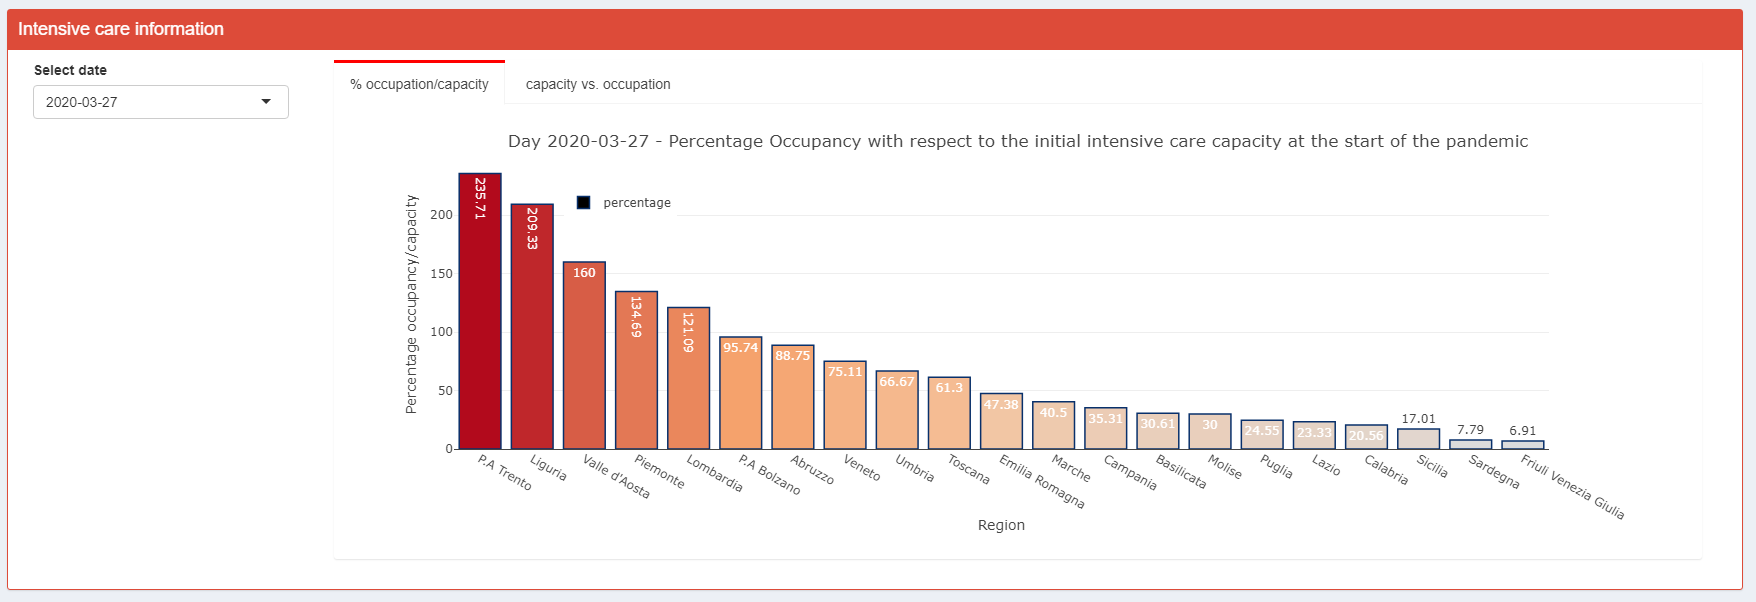
\includegraphics[width=1\linewidth]{Figures/Inspection_perc_occupancy.png}
  \caption{}
  \label{fig:Inspection_perc_occupancy}
\end{subfigure} 
\begin{subfigure}{.8\textwidth}
  \centering
  % include second image
  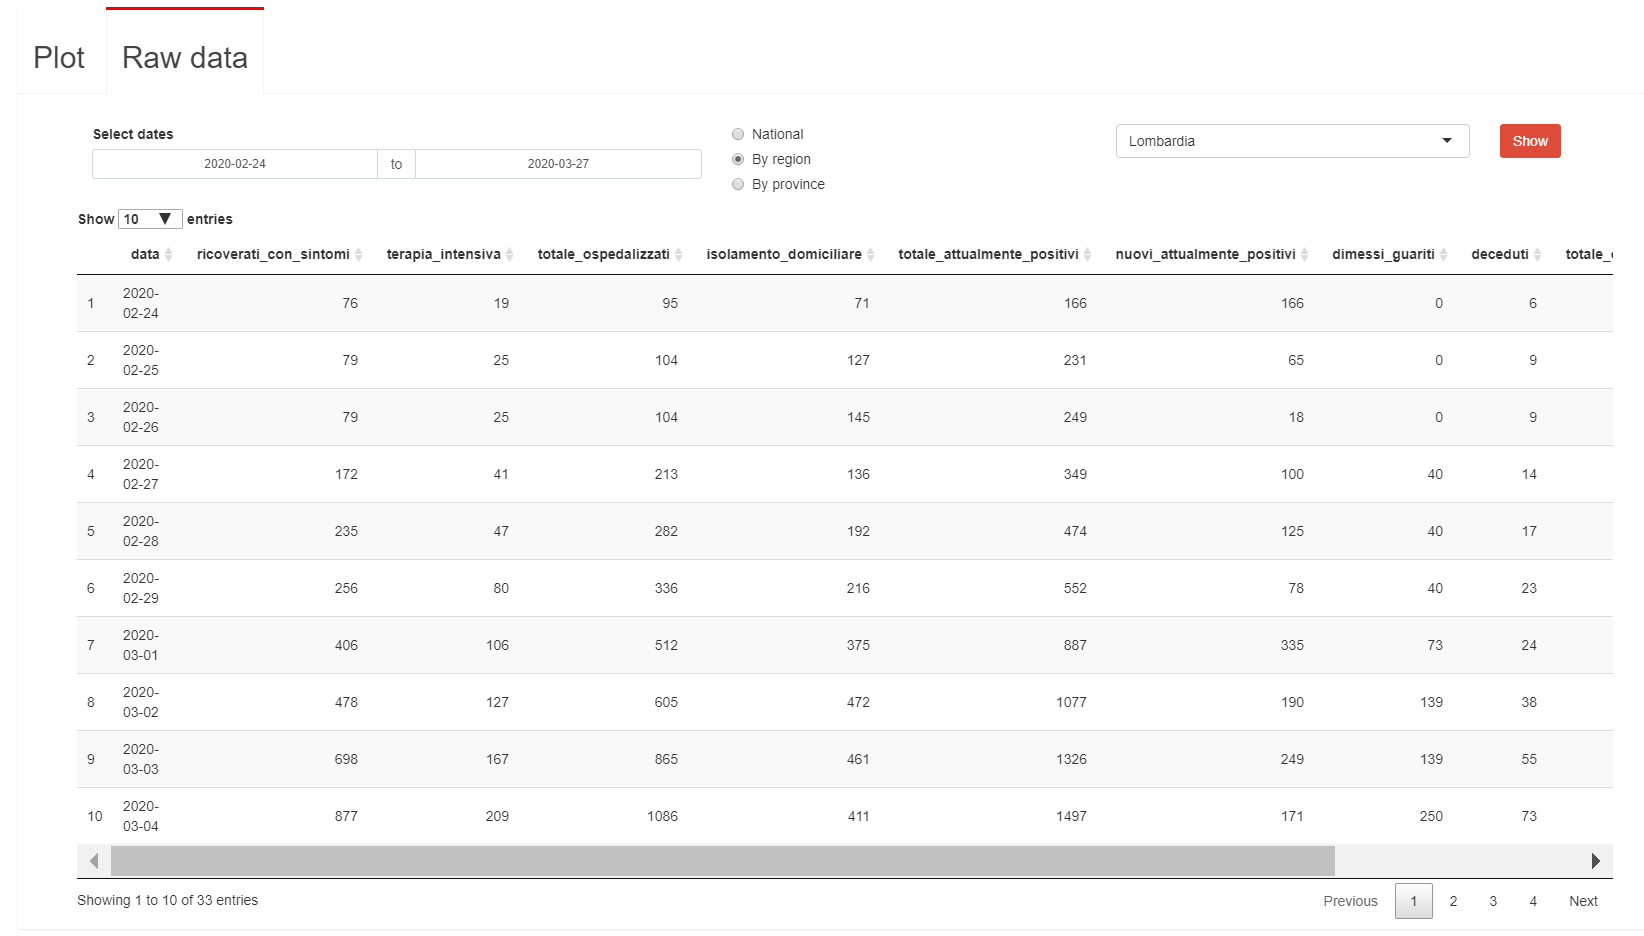
\includegraphics[width=1\linewidth]{Figures/Inspection_rawdata.png} 
  \caption{}
  \label{fig:Inspection_rawdata}
\end{subfigure} 
\begin{subfigure}{.8\textwidth}
  \centering
  % include second image
  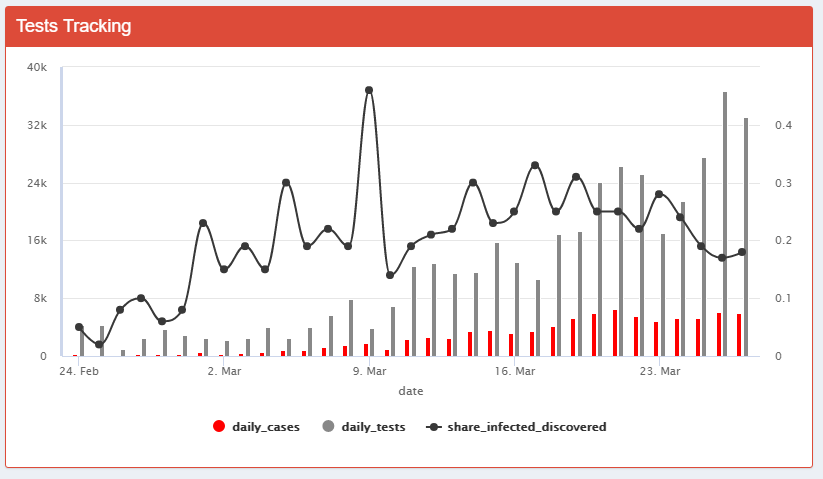
\includegraphics[width=1\linewidth]{Figures/Inspection_test_tracking.png} 
  \caption{}
  \label{fig:Inspection_test_tracking}
\end{subfigure} 
\begin{subfigure}{.8\textwidth}
  \centering
  % include second image
  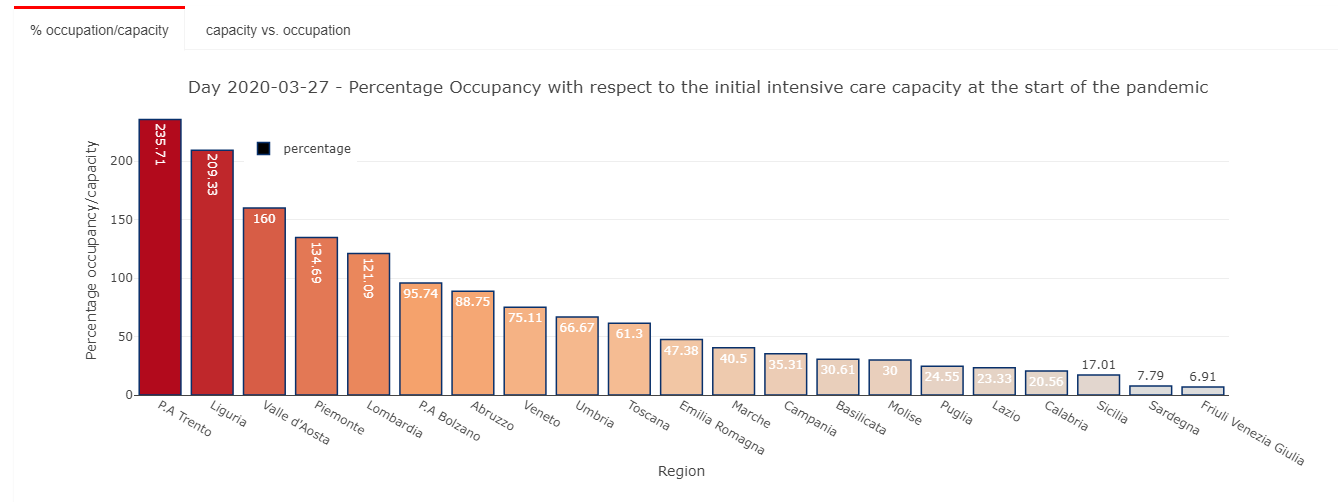
\includegraphics[width=1\linewidth]{Figures/Inspection_Cattura.png} 
  \caption{SEM image of the virus}
  \label{fig:Inspection_Cattura}
\end{subfigure} 
\caption{Subpanels of Data Inspection panel }
\end{figure}

\begin{figure}[H]
  \centering
\begin{subfigure}{0.8\textwidth}
  \centering
  % include second image
  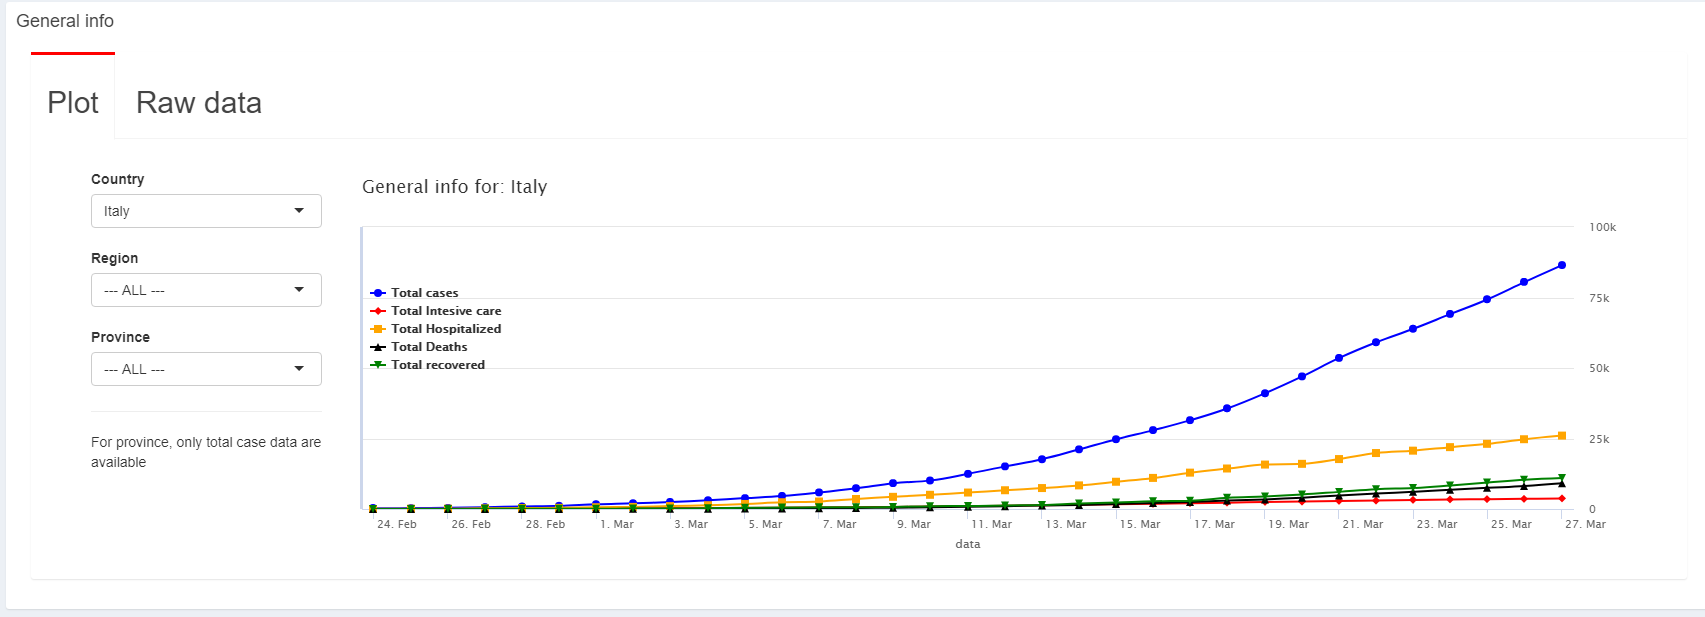
\includegraphics[width=1\linewidth]{Figures/Inspection_general_info.png} 
  \caption{SEM image of the virus}
  \label{fig:Inspection_general_info}
\end{subfigure} 
\begin{subfigure}{0.8\textwidth}
  \centering
  % include second image
  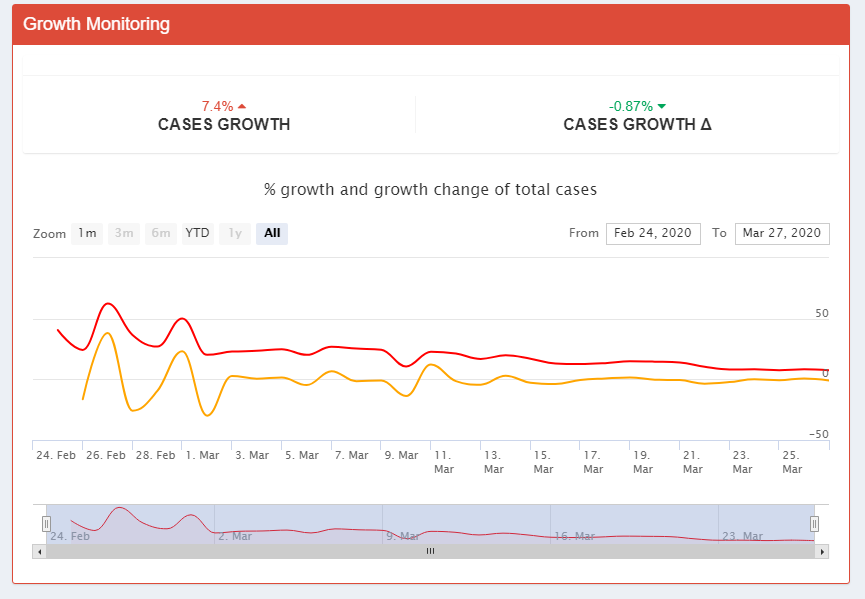
\includegraphics[width=1\linewidth]{Figures/Inspection_growth_monitoring.png} 
  \caption{SEM image of the virus}
  \label{fig:Inspection_growth_monitoring}
\end{subfigure} 
\begin{subfigure}{0.8\textwidth}
  \centering
  % include second image
  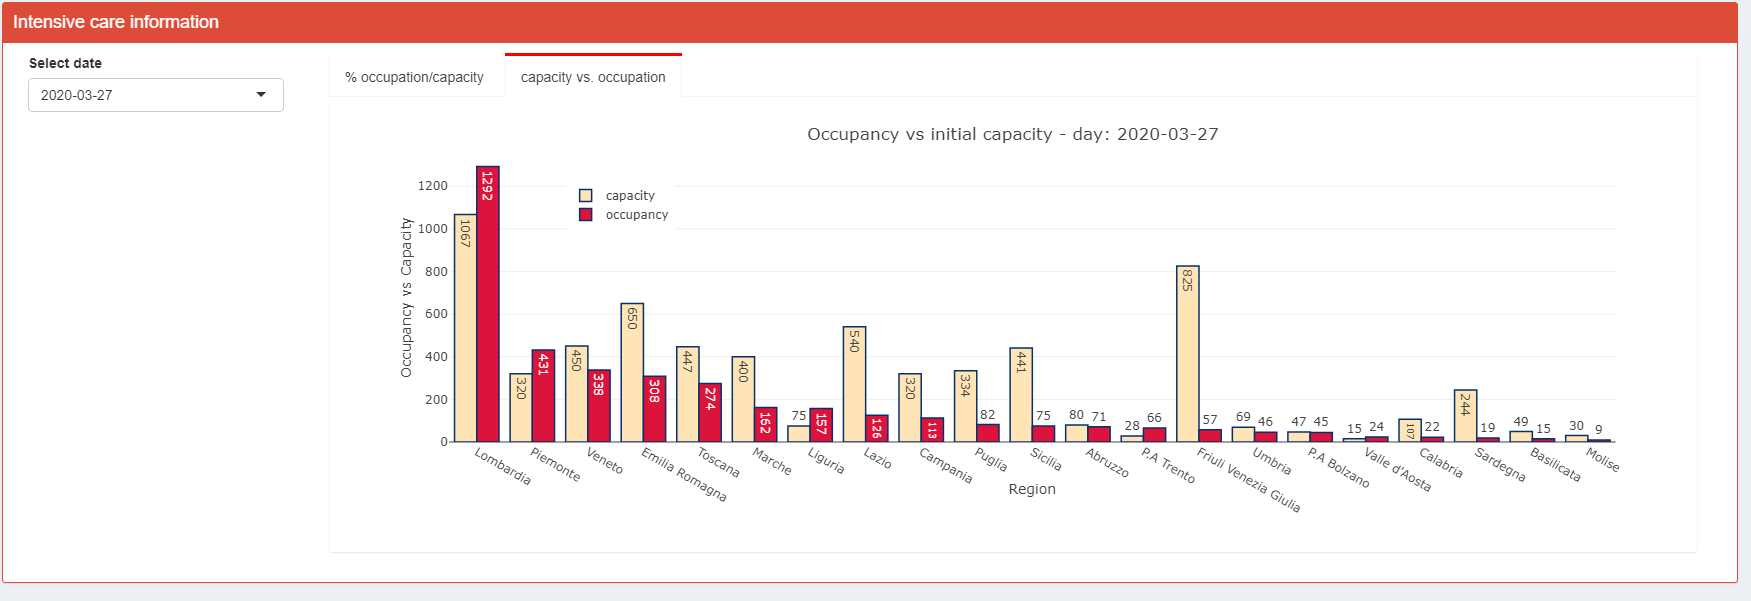
\includegraphics[width=1\linewidth]{Figures/Inspection_occupancy2.png} 
  \caption{SEM image of the virus}
  \label{fig:Inspection_occupancy2}
\end{subfigure}\hspace{0.3\textwidth}
\label{fig:Inspection_panels_2}
\caption{Subpanels of Data Inspection panel }
\end{figure}

\clearpage

\begin{figure}
  \centering
  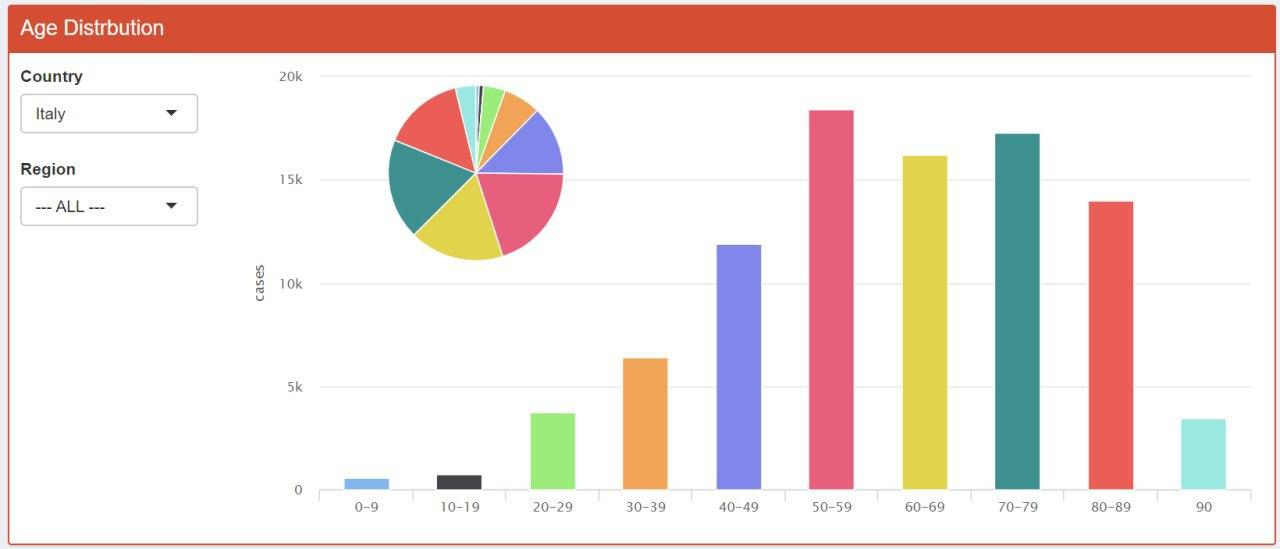
\includegraphics[width=0.8\linewidth]{Figures/Age_distribution.jpg} 
  \caption{The age distribution for the recovered people}
  \label{fig:Age_distribution}
\end{figure}\hspace{0.3\textwidth}


\subsection{Data Analysis}\label{sub:Data Analysis}

Panel \textit{Analysis} explores  several mathematical models for shaping the infection\textquotesingle s time series, namely the ones introduced in Section \ref{Theoretical Background}. As previously argued, each of these model\textquotesingle s predictive power hinges on uncertain actual scenarios, such as the effectiveness of restrictive measures, the presence of several independent and spread outbreaks, and so on.

Package  \cite{growthcurver} has been used for growth curve fitting. This package provides function  \textit{SummarizeGrowth}, which inputs the time series of sample data and outputs the model represented by the growth metrics. Such parameters include those of the logistic equation that best fit the data, namely $K$, $P_0$ and $r$, as in Eq.\ref{logistic_equation}.
The reasons why this package was chosen are chiefly two. At the one hand, it performs non-linear curve fitting with the Levenberg-Marquardt algorithm \cite{more1978levenberg} , which happens to be one of the most robust nls algorithms. For this step, function \cite{nlsLM}  is used. On the other hand, the package is endowed with methods for background correction.

%----> add here packages and documentation for ARIMA <----

At the top of analysis panel the user is allowed to pick one dataset among national, by region and by province. Hence, any following analysis will use the selected dataset as input (the user can browse the raw dataset in panel inspection, see paragraph \ref{Data Inspection} ).

The first section is devoted to the logistic model. An input box (Fig.\ref{fig:logistic_input}) lists several dynamic inputs:
\begin{enumerate}
\item A date range that the calculator will use for curve fitting. The option to choose initial and final dates different from those at, respectively, the beginning and the end of the dataset, is useful in two ways: 
\begin{itemize} 
\item It allows to cut initial dates which possibly correspond to zero or constant infections data, as a consequence of a delay in the outbreak in that territory. Actually, an automatic process will do so after the choice of territory, adjusting the initial date to the first day whose new infections exceed a given threshold (currently set to 1). 
\item It allows to compute the available prediction n days ahead, by cutting the last n dates, and compare it to the real data.
\end{itemize}
\item A check-box \emph{standardise positive cases by total swabs}. If selected, the share of infected among the tested, instead of the infected themselves, will be used for computations and rendering. This may be useful to capture the selection bias, but only in the scenario in which tests are randomly assigned to the population, or at least are assigned with a logic common to all dates and territories. This option is not currently available for provinces.
\item Plot type selection boxes. The available plot types are cumulative cases and new cases. (The user can always show and hide plot\textquotesingle  s components by clicking on their label in the legend).
\item Residuals plot type. Four options for graphically rendering the residuals: Residuals vs. fitted values; Standardized residuals vs. fitted values; Autocorrelation; Square root of absolute residuals vs. fitted values.
\end{enumerate}

The output is displayed within three boxes: 
\begin{enumerate}
\item Inside the \ref{fig:logistic_plot1} box the sample points, the fitted logistic curve and a confidence band at 95 \% level for the logistic curve are overlayed. The user can view the sample and fitted values by hovering over or touching (for touch-screen devices) them \ref{fig:logistic_plot1}. In addition, if \emph{new cases} is selected, a plot of sample cases differences (which correspond to new cases, in fact) is shown over the logistic estimated distribution \ref{fig:logistic_plot2}.. The latter is simply obtained by deriving the right hand side of formula $(4.3.1)$:
\begin{equation}
N'(t) = \frac{(\frac{K-N_0}{N_0})Kre^{-rt}}{[1+(\frac{K-N_0}{N_0})e^{-rt}]^2}
\end{equation}
The user is suggested to take full advantage of plotly features. Besides showing points labels when passing over it and enabling plot selection by clicking on label items, plotly charts are endowed with a sequence of tools shown at the top-right of the box \ref{fig:logistic_plot3}.
\item Summary output box \ref{fig:logistic_smry1} contains principal information about the selected model and a list of goodness-of-fit tests on the residuals. 
\item Residuals box contains the plots of residuals, rendered in the user-chosen fashion. (see Fig.\ref{fig:logistic_res1}).
\end{enumerate}

\begin{figure}[H]
  \centering
\begin{subfigure}{0.6\textwidth}
  % include second image
  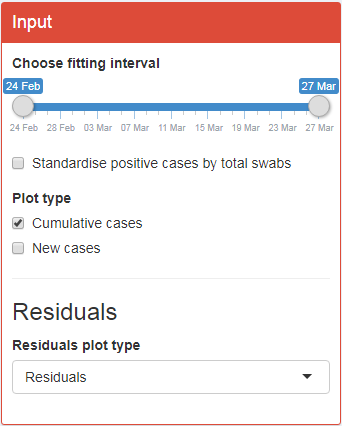
\includegraphics[width=1\linewidth]{Figures/logistic_input.png} 
  \caption{Input box of the logistic curve section.}
  \label{fig:logistic_input}
\end{subfigure} 
\hspace{5.5cm}
\begin{subfigure}{0.6\textwidth}
  % include second image
  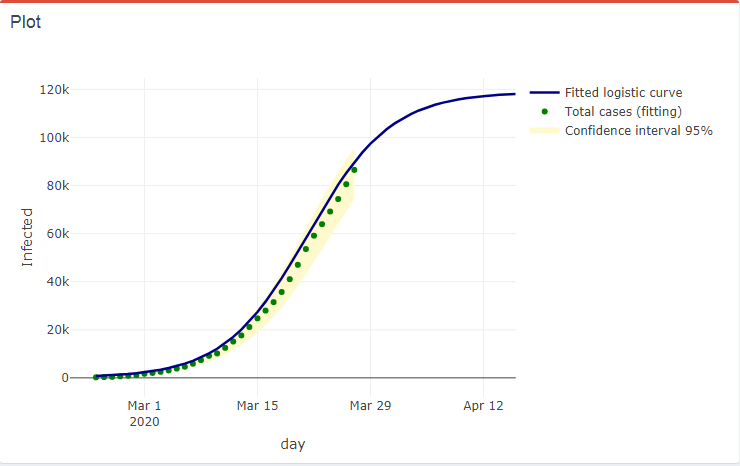
\includegraphics[width=1\linewidth]{Figures/logistic_plot1.png} 
  \caption{ Plot of fitted logistic curve over sample cumulative cases of infection, plus a 95 \% confidence band. Green points are the observed data used for fitting, red ones are the remaining. Hovering over any point or curve displays info such as x and y coordinates.}
  \label{fig:logistic_plot1}
\end{subfigure} 
\hspace{5.5cm}
\begin{subfigure}{0.6\textwidth}
  % include second image
  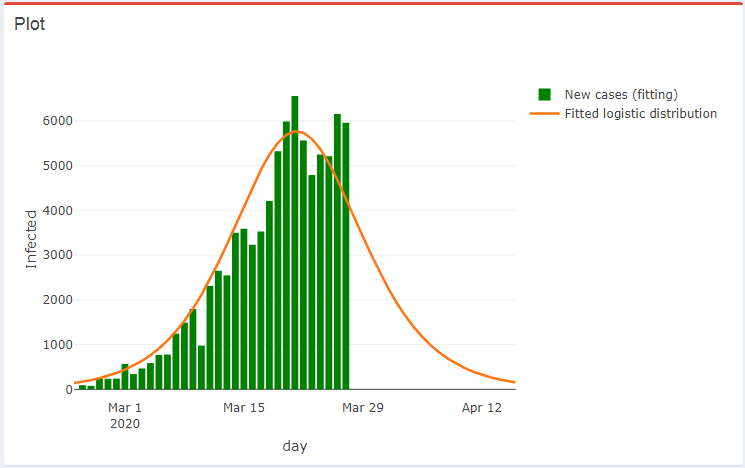
\includegraphics[width=1\linewidth]{Figures/logistic_plot2.png} 
  \caption{Plot of estimated logistic distribution over sample new cases of infection.}
  \label{fig:logistic_plot2}
\end{subfigure}
\label{fig:logistic_plots_set}
\caption{Subpanels of Data Analysis panel }
\end{figure}


\begin{figure}[H]
  \centering
\begin{subfigure}{0.6\textwidth}
  % include second image
  
\includegraphics[width=1\linewidth]{Figures/logistic_plot3.png} 
  \caption{SSet of useful tools for navigating into plots, by plotly.}
  \label{fig:logistic_plot3}
\end{subfigure} 
\hspace{5.5cm}
\begin{subfigure}{0.6\textwidth}
  % include second image
  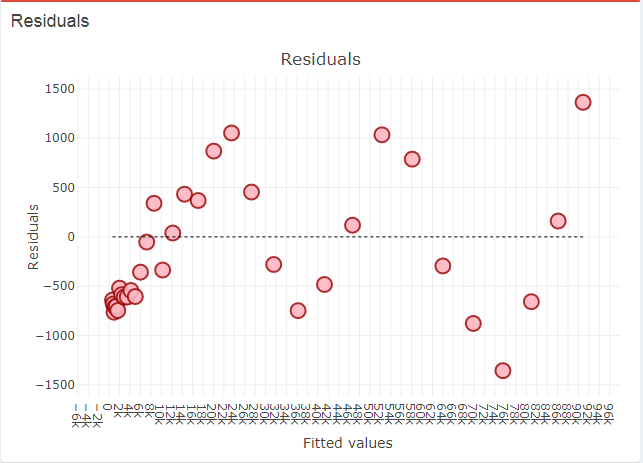
\includegraphics[width=1\linewidth]{Figures/logistic_res1.png} 
  \caption{One plot of nls residuals: square root of absolute residuals vs. fitted values.}
  \label{fig:logistic_res1}
\end{subfigure} 
\hspace{5.5cm}
\begin{subfigure}{0.6\textwidth}
  % include second image
  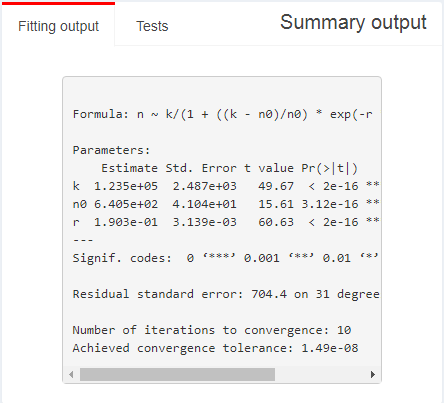
\includegraphics[width=1\linewidth]{Figures/logistic_smry1.png} 
  \caption{Summary output box of logistic section.}
  \label{fig:logistic_smry1}
\end{subfigure}
\label{fig:logistic_plots_set2}
\caption{Subpanels of Data Analysis panel }
\end{figure}

\clearpage

\section{Conclusions}

\section{Packages used}


%------------------------------------------------



%----------------------------------------------------------------------------------------
%	BIBLIOGRAPHY
%----------------------------------------------------------------------------------------

\renewcommand{\refname}{\spacedlowsmallcaps{References}} % For modifying the bibliography heading

\bibliographystyle{unsrt}

\bibliography{sample.bib} % The file containing the bibliography

%----------------------------------------------------------------------------------------

\end{document}